\chapter{Evaluation}

\section{Customer Requirements}

For this section I will be evaluating whether or not my system has met my initial objectives that were proposed in the Analysis section. This will be used to determine whether or not the system has met the customer requirements. If the system does not meet an objective then I will include a further explanation of why this is the case. If the objective has been met then I will provide evidence to support this evaluation.

The objectives have been split into:
\begin{itemize}
\item{General Objectives}
\item{Specific Objectives}
\item{Core Objectives}
\item{Other Objectives}
\item{Additional Objectives}
\end{itemize}

Some of the objectives overlap into other sections, the overlapping objectives I have only included once.

%include as many subsections as necessary for your objectives
\paragraph{General Objectives}

\subsection{Database Functionality}\label{staffhardware}

\textbf{Objective:} A database to show all current staff (with details such as their job title) and the hardware devices they are assigned to.

\textbf{Has the objective been fulfilled?}

This objective has been fulfilled. I have met this objective by examining the company's current spreadsheet (their current way to store data) and making sure that all the correct fields were included in my database. To display allocation of hardware devices to staff members it was important to make the database relational, this was done with the use of primary and foreign keys. Using this method means hardware can be added to a separate table to staff and then linked in the StaffHardware table which the staff members will see. My client strongly agrees that all devices in this table are shown correctly (question 14 \ref{qs}, page \pageref{qs}).

\textbf{Evidence}

Below are the different interfaces that will present the database that shows current staff and their assigned hardware devices.

\begin{figure}[H]
    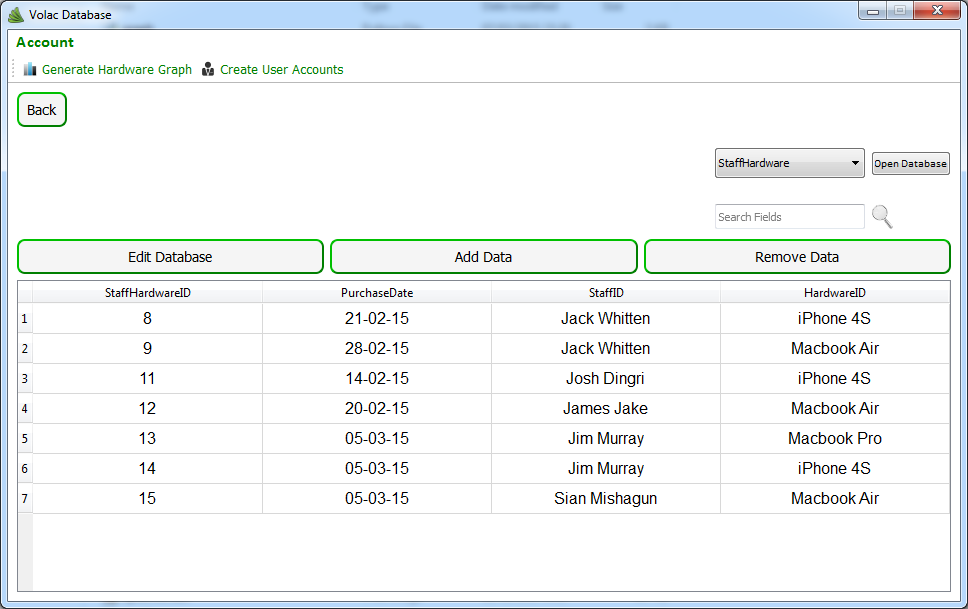
\includegraphics[width=\textwidth]{./Evaluation/Images/Database1.png}
    \caption{The Admin interface, viewing the StaffHardware Table.} \label{fig:db1}
\end{figure}

\begin{figure}[H]
    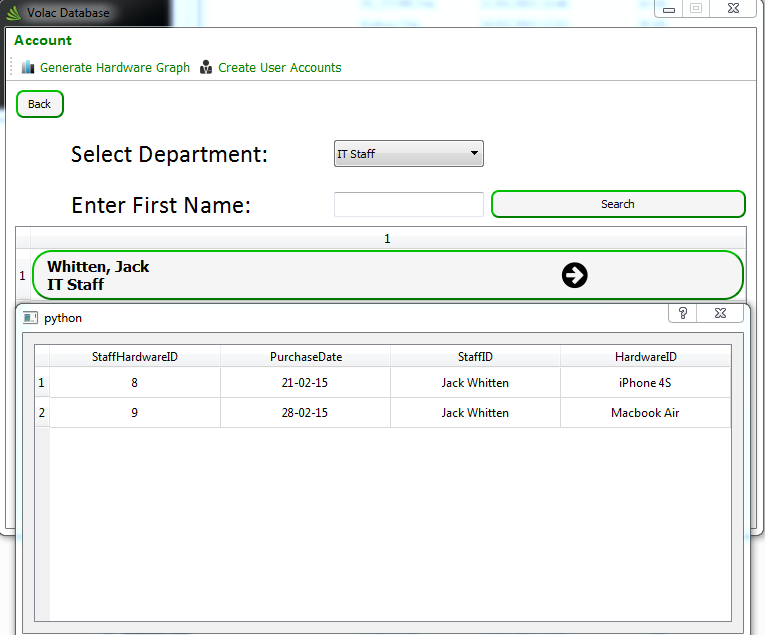
\includegraphics[width=\textwidth]{./Evaluation/Images/database3.png}
    \caption{The Admin interface: When searching for data and clicking to view more information, the StaffHardware table will appear.} \label{fig:db2}
\end{figure}

\begin{figure}[H]
    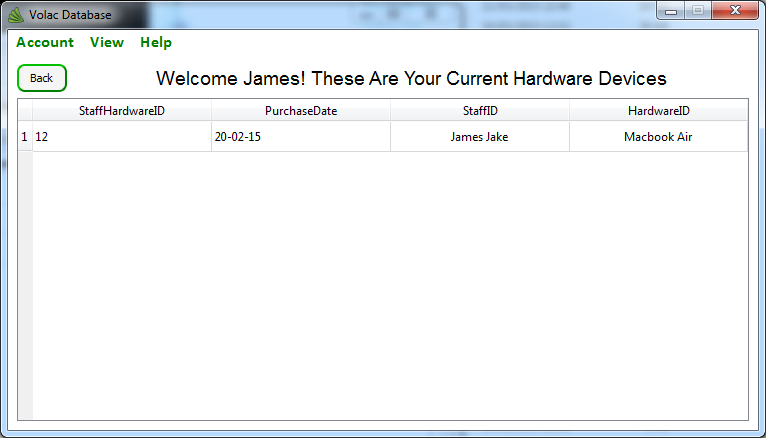
\includegraphics[width=\textwidth]{./Evaluation/Images/database2.png}
    \caption{The Manager (and staff) interface, viewing their current hardware devices.} \label{fig:db3}
\end{figure}

\subsection{Clear Database Structure}

\textbf{Objective:} The database will replace the current spreadsheet and be easy to read as information will be clear and organized.

\textbf{Has the objective been fulfilled?}

The objective has been met. The database includes all the needed fields from the spreadsheet and makes use of drop down boxes to make data organised. Each table is viewed by selecting it from the drop down box which means there is not too much information on the screen at one time. The font size was increased so the data is easy to read and the system has been spaced out so information is not cluttered.

\textbf{Evidence}

\begin{figure}[H]
    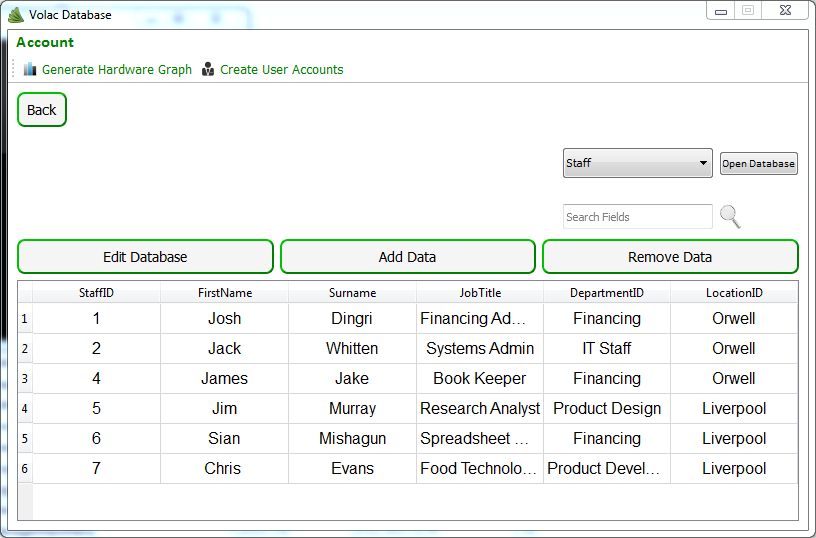
\includegraphics[width=\textwidth]{./Evaluation/Images/cleardb1.png}
    \caption{Easily readable font size with clear headers for the fields.}
\end{figure}

\begin{figure}[H]
    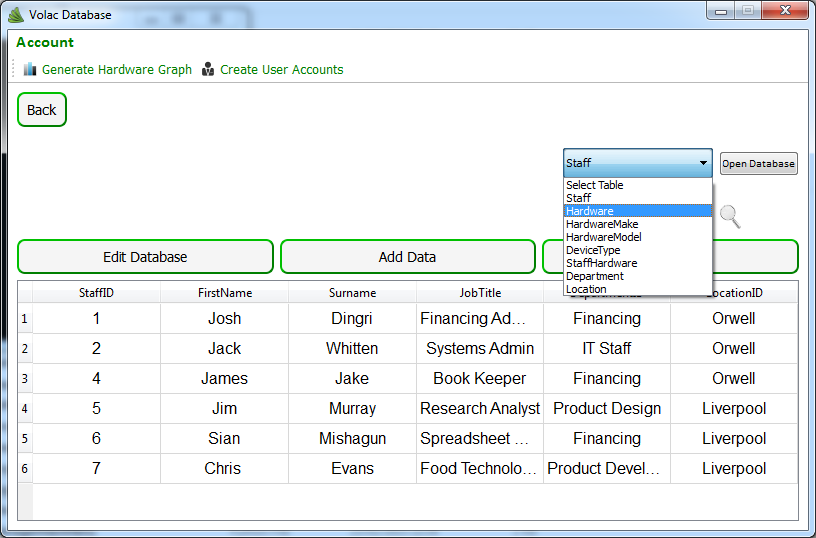
\includegraphics[width=\textwidth]{./Evaluation/Images/cleardb2.png}
    \caption{The dropdown box allows the user to choose which table to view which shows its organisation} 
\end{figure}

\begin{figure}[H]
    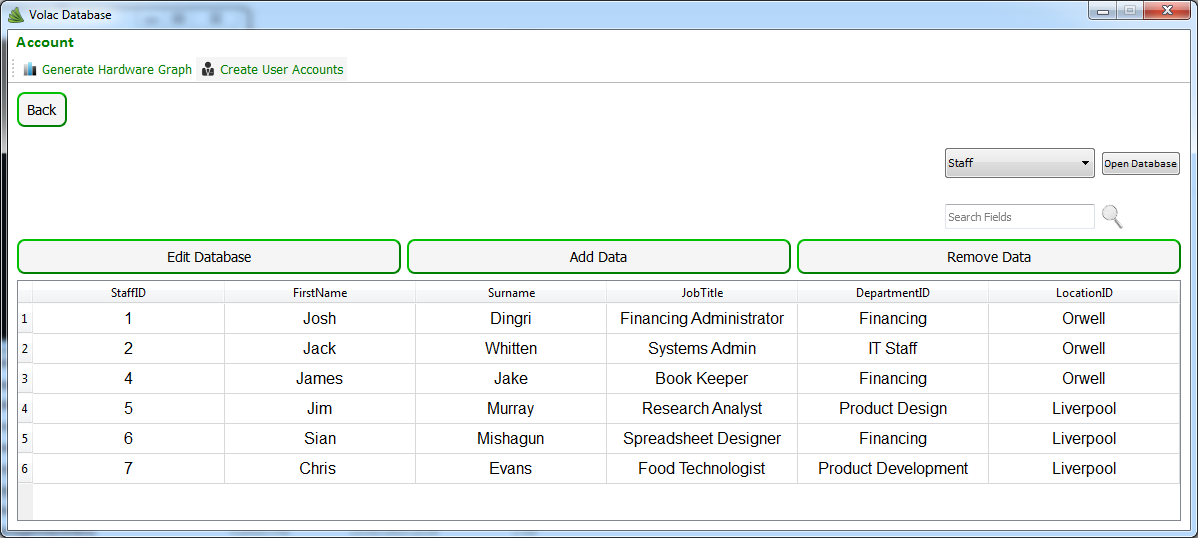
\includegraphics[width=\textwidth]{./Evaluation/Images/cleardb3.png}
    \caption{The table (with the application) can be resized to view all fields. It can only be resized to a certain point because otherwise the layout of the application becomes stretched and there is no real need to stretch it past the maximum point.} 
\end{figure}


\subsection{Easy to use Data Input and Keyboard Shortcuts}

\textbf{Objective:} An easy to use database for IT staff to enter colleague data with toolbar buttons and keyboard shortcuts as they are advanced computer users and will want an quicker way of doing things.

\textbf{Has the objective been fulfilled?}

The objective has been fulfilled. There are toolbar buttons on the admin interface to allow account and graph generations. There are also keyboard shortcuts that are linked to some of the menubar buttons so staff can use them quickly, for example using F1 and F2 (for managers) to switch between layouts. Some of the shortcuts suggested in the design have been left out, the user will not be able to choose a table to edit from the menubar. My client liked the keyboard shortcuts and strongly agreed that they would help complete tasks quicker (question 5 \ref{qs}, page \pageref{qs}).

\textbf{Evidence}

\begin{figure}[H]
    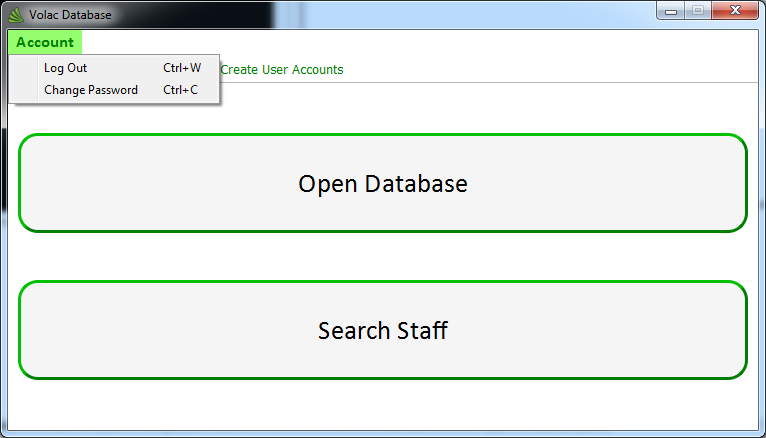
\includegraphics[width=\textwidth]{./Evaluation/Images/shortcuts1.png}
    \caption{The menu buttons can be activated by using the menubar or some (such as the above) have keyboard shortcuts attached to them.} 
\end{figure}

\begin{figure}[H]
    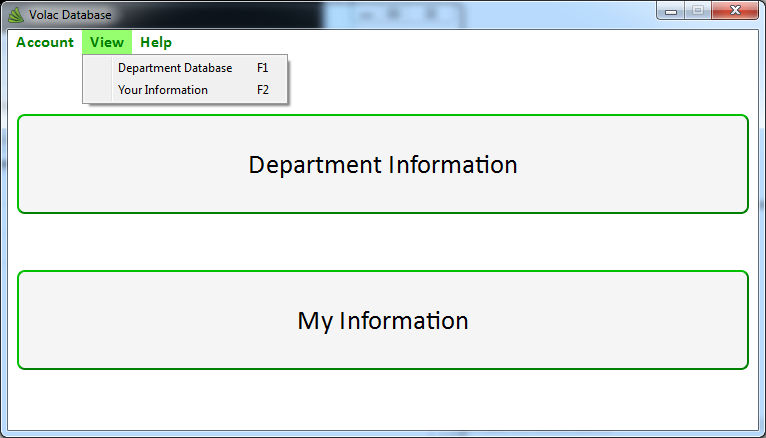
\includegraphics[width=\textwidth]{./Evaluation/Images/shortcuts2.png}
    \caption{This menu is part of the Manager interface showing F1 and F2 shortcuts which are attached to the menu buttons.} 
\end{figure}


\subsection{Simple Interface Structure}\label{interface}

\textbf{Objective:} The layout for colleagues to see their hardware allocations will be clear and to the point, missing out any unnecessary buttons and menus.

\textbf{Has the objective been fulfilled?}

The objective has been fulfilled. I have ensured that there is not too many buttons on the system and that all buttons are clearly labeled. I did not include a menu from the design because it was unnecessary. For the staff interface they have a simply table showing their devices  since they do not need any extra features. 

\textbf{Evidence}

\begin{figure}[H]
    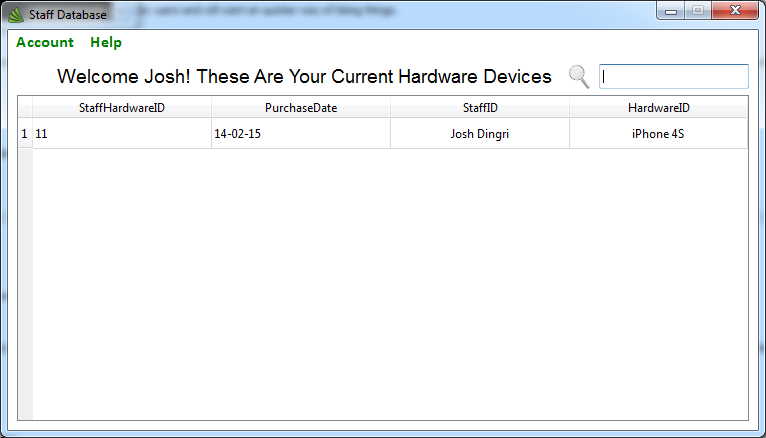
\includegraphics[width=\textwidth]{./Evaluation/Images/staffhardwaredevice.png}
    \caption{A simple view of the Staff interface showing a user's hardware items.} 
\end{figure}

\begin{figure}[H]
    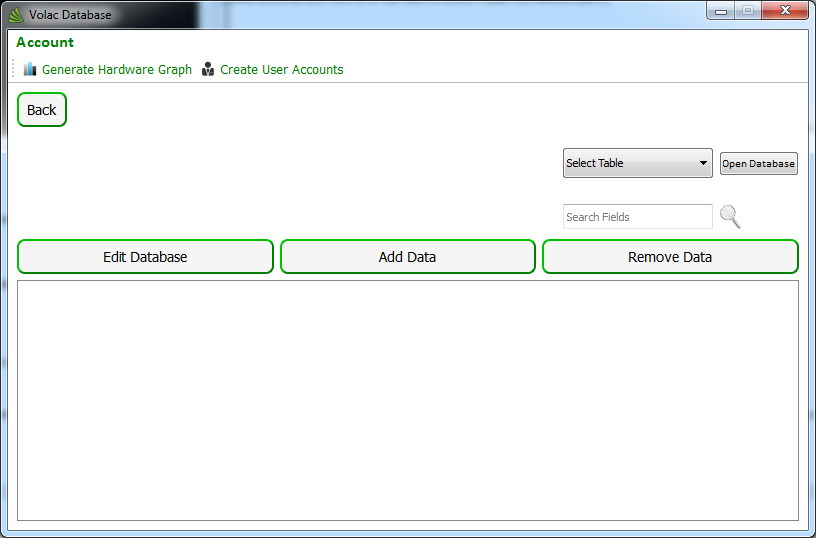
\includegraphics[width=\textwidth]{./Evaluation/Images/clearlabels.png}
    \caption{A view of the Admin interface before a database is selected. All buttons are clearly labelled and the screen is not cluttered.} 
\end{figure}


\subsection{Search Functionality}\label{search}

\textbf{Objective:} A search function will be in place to make searching for a field (such as staff member or hardware device) easy.

\textbf{Has the objective been fulfilled?}

The objective has been fulfilled. There are search functions on every interface which enables staff to easily search the table. The admin interface also has a more advanced search which allows them to search for staff members by department and then click to view more information about their colleague. The basic search function on each table allows users to search for any field in the table, simply by entering text into the search box the table will automatically search for the data. My client strongly agreed that the search function very easy to use (question 17 \ref{qs}, page \pageref{qs}).

\textbf{Evidence}

\textbf{Admin Database Screen}

\begin{figure}[H]
    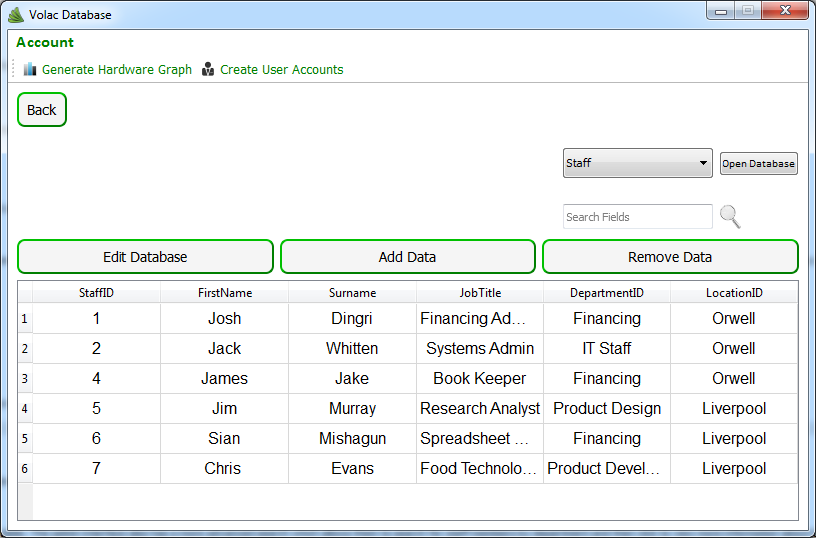
\includegraphics[width=\textwidth]{./Evaluation/Images/beforeadminsearch.png}
    \caption{A view of the admin database screen before any data is searched.} 
\end{figure}


\begin{figure}[H]
    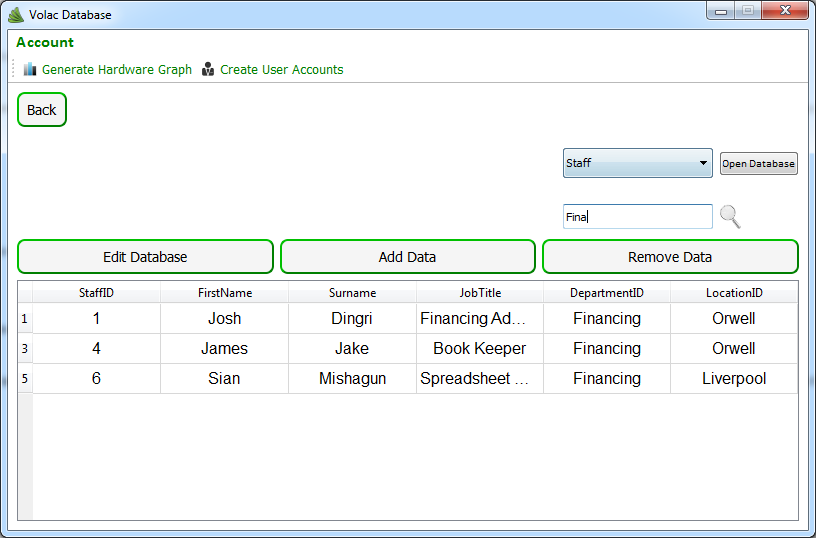
\includegraphics[width=\textwidth]{./Evaluation/Images/afteradminsearch.png}
    \caption{A view of the admin database screen after data is searched.} 
\end{figure}

\textbf{Admin Staff Search Screen}

\begin{figure}[H]
    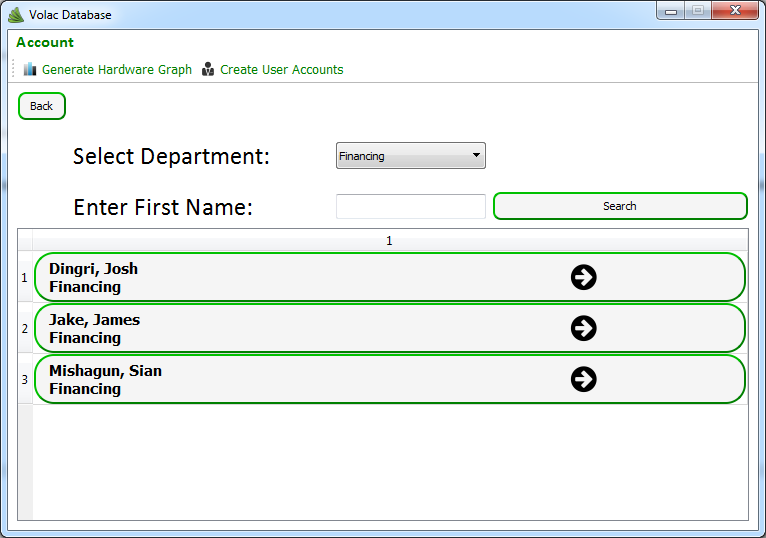
\includegraphics[width=\textwidth]{./Evaluation/Images/beforeadv.png}
    \caption{A view of the admin "search staff" screen before member is searched.} 
\end{figure}

\begin{figure}[H]
    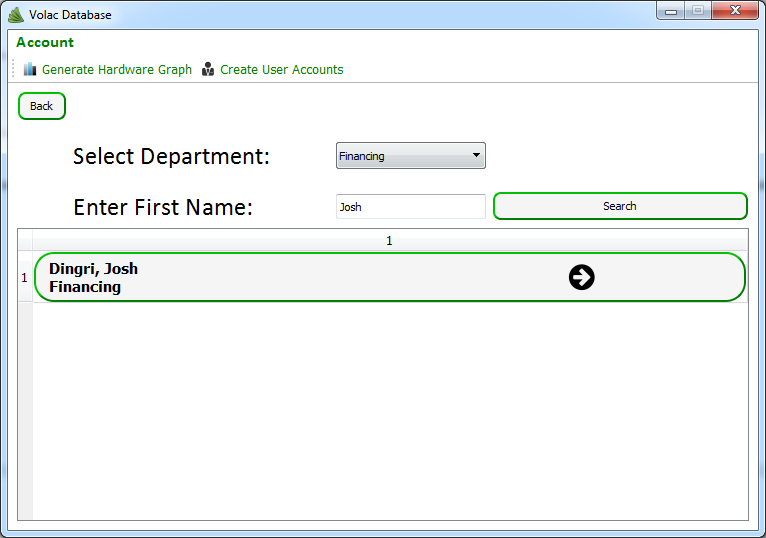
\includegraphics[width=\textwidth]{./Evaluation/Images/afteradv.png}
    \caption{A view of the admin "search staff" screen after member is searched.} 
\end{figure}

\textbf{Manager Search}

\begin{figure}[H]
    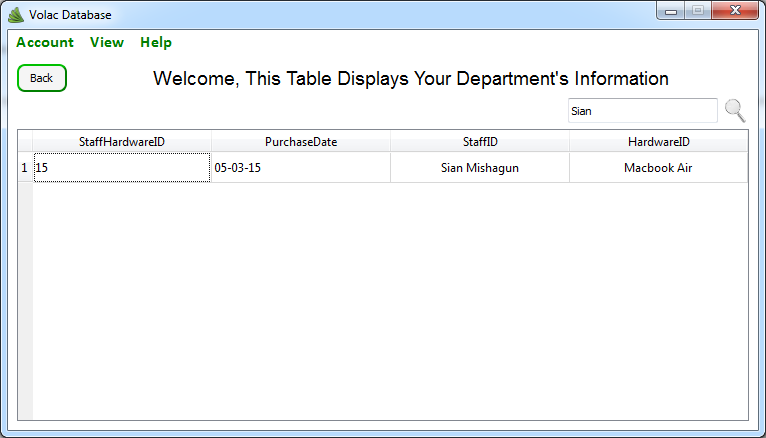
\includegraphics[width=\textwidth]{./Evaluation/Images/managersearch.png}
    \caption{A view of the manager table when data is searched.} 
\end{figure}

\textbf{Staff Search}

\begin{figure}[H]
    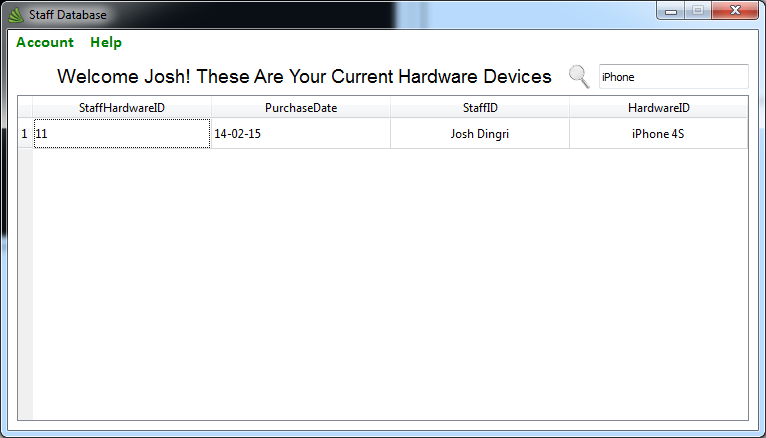
\includegraphics[width=\textwidth]{./Evaluation/Images/staffsearch.png}
    \caption{A view of the staff table when data is searched.} 
\end{figure}

\begin{figure}[H]
    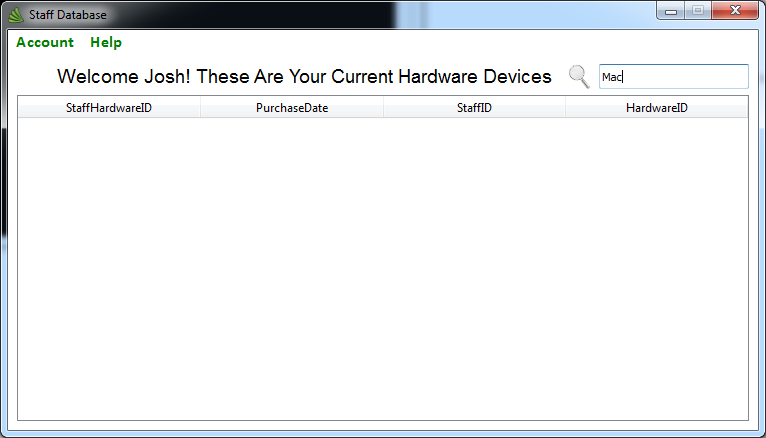
\includegraphics[width=\textwidth]{./Evaluation/Images/staffsearch2.png}
    \caption{A view of the staff table when data is searched but no fields match.} 
\end{figure}



%%%%
\paragraph{Specific Objectives}

\subsection{Tables}

\textbf{Objective:}The database will have one table with staff and a relationship to the table with their hardware device. This will show which hardware devices the staff are allocated and all the details of that hardware device. Staff details including department and location will be linked to the Department and Location tables.

\textbf{Has the objective been fulfilled?}

The objective has been met. All relationships have been made successfully which reduces data duplication and some fields can be chosen simply by selecting from drop down boxes. The StaffHardware table (linking staff with hardware devices) is present on each interface since this is the most important and main table for viewing allocated hardware devices.

\textbf{Evidence}

See \ref{staffhardware} (page: \ref{staffhardware}) for StaffHardware tables.

\begin{figure}[H]
    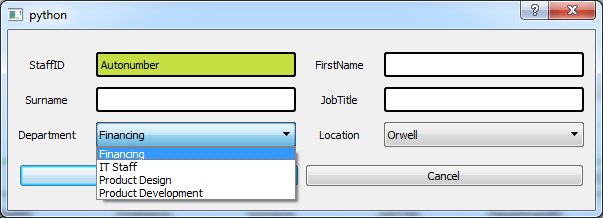
\includegraphics[width=\textwidth]{./Evaluation/Images/dropdown.png}
    \caption{A dropdown box showing how data duplication is avoided. This also shows the link to the department table.} 
\end{figure}



\subsection{How the System will Search for Data}

\textbf{Objective:}The search function will allow a user to enter text and will highlight where on the page that text is.

\textbf{Has the objective been fulfilled?}

This specific objective has not been met, but has instead been improved. The reason for this is that I have changed how the search function works. It was not efficient to have to data be highlighted when the user enters text because if there was a lot of data it would still be hard to find the highlighted text. I have changed this so the table only shows the data that meets the search criteria, all other records will be hidden. For example if the user was to search for "Financing" all the staff members from the Financing department would be shown.

\textbf{Evidence}

See \ref{search} (page: \pageref{search}) for evidence of the search function.


\subsection{Read-Only access for staff}

\textbf{Objective:} Read-Only access for staff viewing their own information (with a log-in system to allow this).

\textbf{Has the objective been fulfilled?}

This objective has been met. The lowest access level (for normal staff use) displays the "StaffHardware" table in read only format, which means no data can be modified. The login system allows the staff to log in to their interface, each interface has its own access restrictions. In order of how much access received, the interfaces are Admin, Manager and Staff. My client strongly agreed that the access levels were correct in the system (question 11 \ref{qs}, page \pageref{qs}).

\textbf{Evidence}

\begin{figure}[H]
    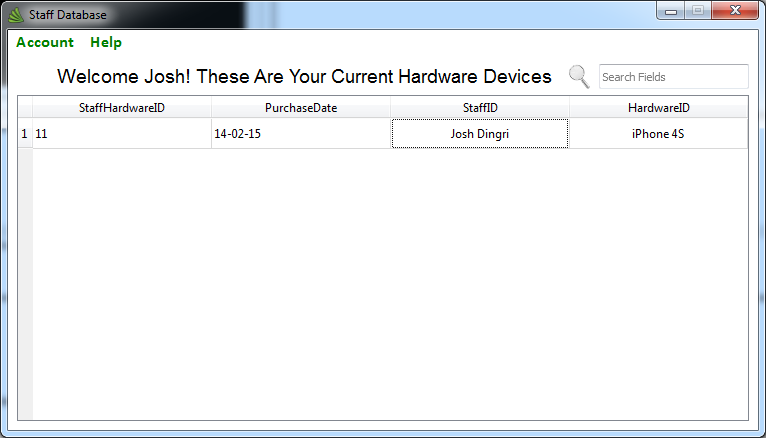
\includegraphics[width=\textwidth]{./Evaluation/Images/readonlystaff.png}
    \caption{The grey box around the field shows up meaning that the field cannot be modified.} 
\end{figure}



\subsection{Read-Only access for managers}

\textbf{Objective:}Read-Only access for line managers wanting to see all data about staff in their department.

\textbf{Has the objective been fulfilled?}

This objective has been fulfilled. Managers have read only access to the table which displays information about their department.

\textbf{Evidence}

\begin{figure}[H]
    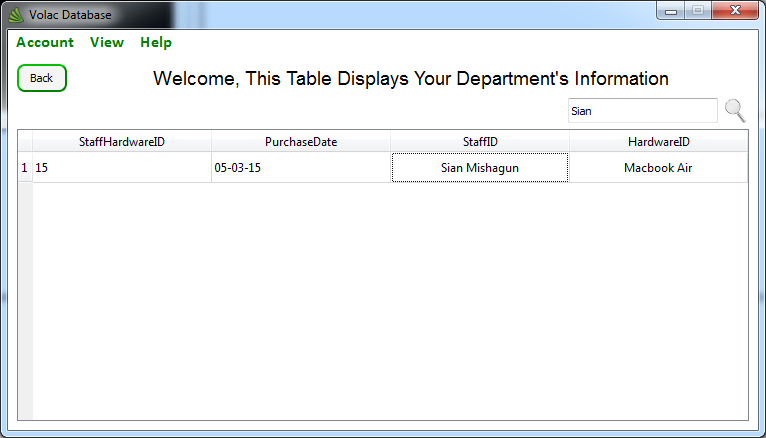
\includegraphics[width=\textwidth]{./Evaluation/Images/readonlymanager.png}
    \caption{The grey box around the field shows up meaning that the field cannot be modified.} 
\end{figure}




\subsection{Admin access for IT Staff}\label{admin}

\textbf{Objective:}Admin rights for IT staff so they are able to view and edit all data on the database.

\textbf{Has the objective been fulfilled?}

Objective has been fulfilled. Admin access allow the user to  view all of the tables in the database in order to add, edit and remove any data. When creating log in accounts, the user can give admin access to any staff member, so when the company come to use the system it may not be just IT Staff as the objective says.

\textbf{Evidence}

\begin{figure}[H]
    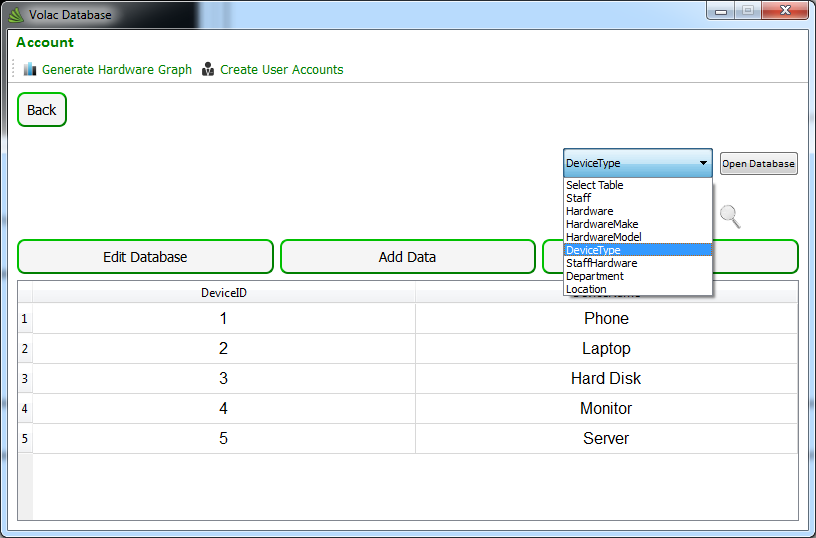
\includegraphics[width=\textwidth]{./Evaluation/Images/admin1.png}
    \caption{Admin Interface showing that all tables can be viewed in the database.} 
\end{figure}

\begin{figure}[H]
    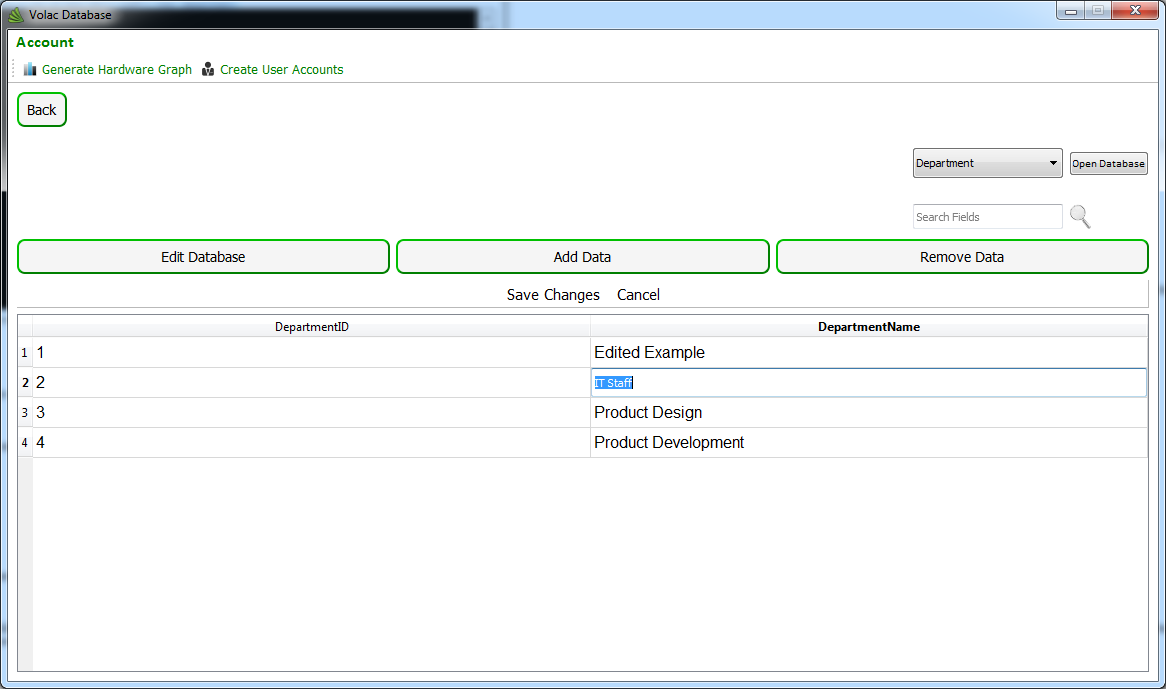
\includegraphics[width=\textwidth]{./Evaluation/Images/admin2.png}
    \caption{Admin Interface showing that data can be edited.} 
\end{figure}

\begin{figure}[H]
    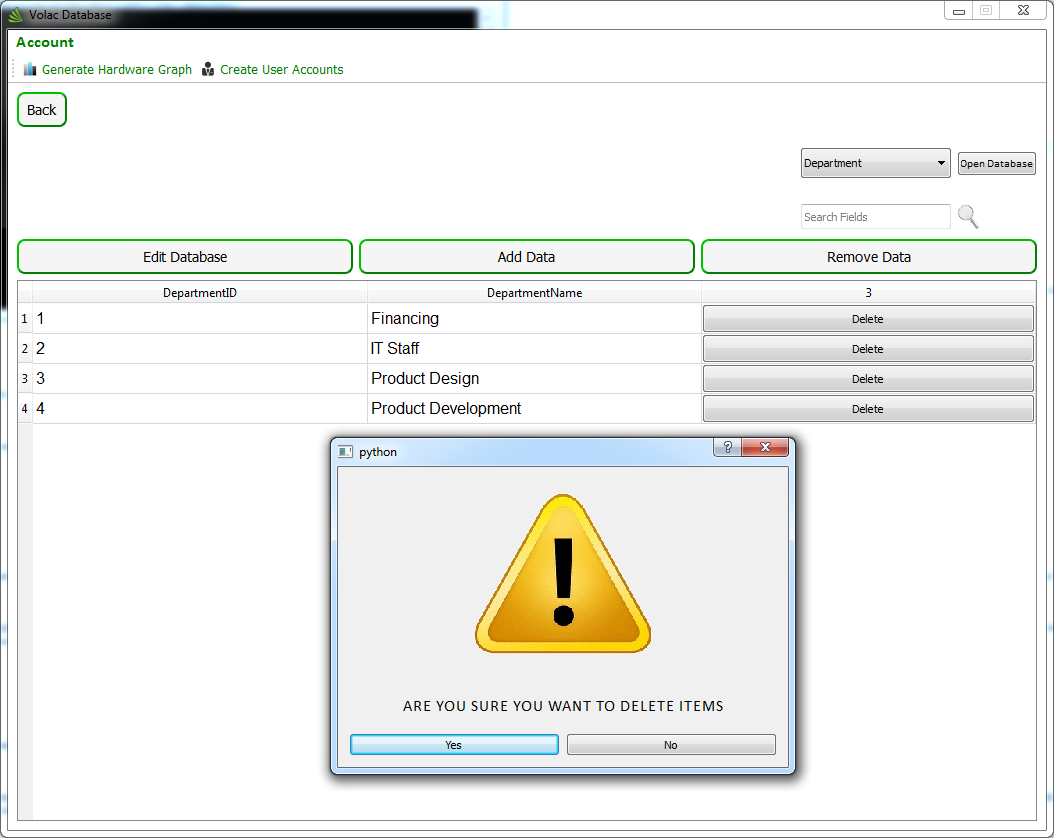
\includegraphics[width=\textwidth]{./Evaluation/Images/admin3.png}
    \caption{Admin Interface showing that data can be deleted.} 
\end{figure}



\subsection{Querying Data}

\textbf{Objective:} Users will be able to query information, for example if they wanted to show only mobile phones or if they wanted to show only specific departments.

\textbf{Has the objective been fulfilled?}

The objective has been met by using the search functions on each table but there is no advanced way to query data, apart from using the admin interface to search for staff by department. 

\textbf{Evidence}

The search function shown in section \ref{search}(page: \pageref{search})

The below screenshots show querying by department.

\begin{figure}[H]
    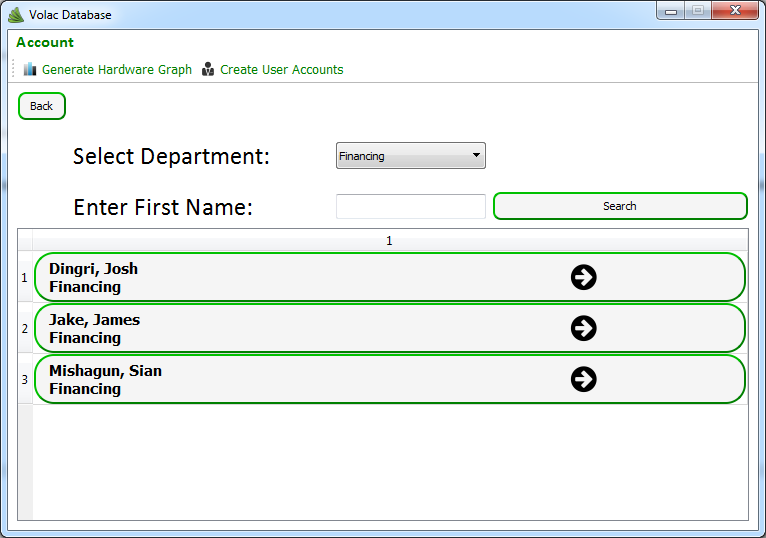
\includegraphics[width=\textwidth]{./Evaluation/Images/beforeadv.png}
    \caption{A view of the admin "search staff" screen before member is searched.} 
\end{figure}

\begin{figure}[H]
    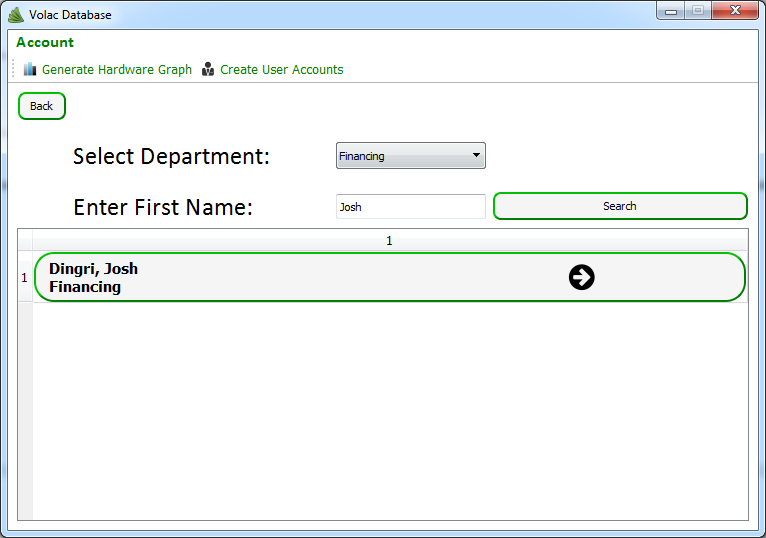
\includegraphics[width=\textwidth]{./Evaluation/Images/afteradv.png}
    \caption{A view of the admin "search staff" screen after member is searched.} 
\end{figure}



\paragraph{Core Objectives}

\subsection{The Login System}

\textbf{Objective:}The system will provide a login system where IT staff can assign usernames to all staff and have admin rights to view all data. The database will have read-only access for colleagues viewing their own information. Managers will be able to view their departments hardware devices.

\textbf{Has the objective been fulfilled?}

Objective has been fulfilled. IT Staff (or admins) can successfully create usernames and password for other staff members that they can then use to log in to the system with. Admins can also view all tables in the database and add, edit and remove data. Managers can log in the their interface where they can view their departments data along with their own hardware devices. Other staff can log in to the basic interface that will allow them to view their own data. My client strongly agreed that the access levels were correct in the system (question 11 \ref{qs}, page \pageref{qs}).

\textbf{Evidence}

\begin{figure}[H]
    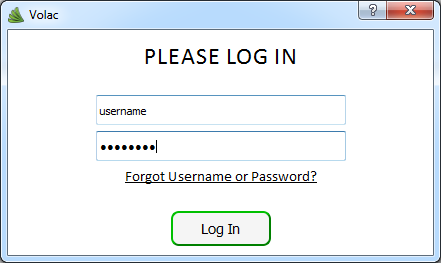
\includegraphics[width=\textwidth]{./Evaluation/Images/login1.png}
    \caption{Admin Interface showing account creation, from here they can choose access levels for other staff members to use.} 
\end{figure}

\begin{figure}[H]
    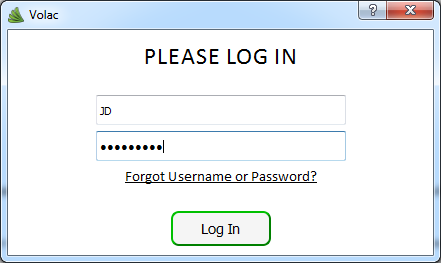
\includegraphics[width=\textwidth]{./Evaluation/Images/login2.png}
    \caption{Example of admin login.} 
\end{figure}

\begin{figure}[H]
    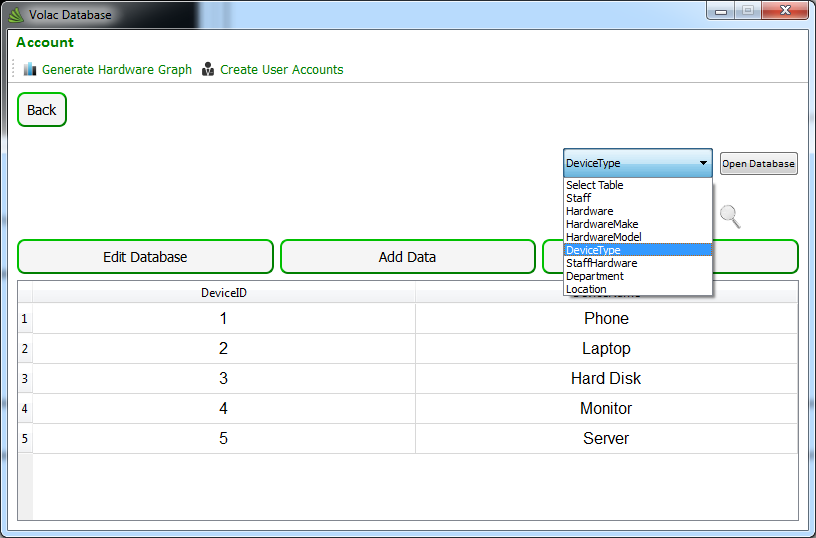
\includegraphics[width=\textwidth]{./Evaluation/Images/admin1.png}
    \caption{Admin Interface showing that all tables can be viewed in the database. (see \ref{admin} (page: \pageref{admin})for editing and removing data)}
\end{figure}

\begin{figure}[H]
    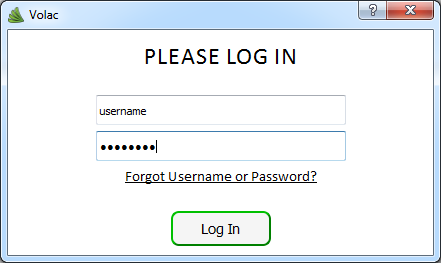
\includegraphics[width=\textwidth]{./Evaluation/Images/login3.png}
    \caption{A view of the admin "search staff" screen after member is searched.} 
\end{figure}

\begin{figure}[H]
    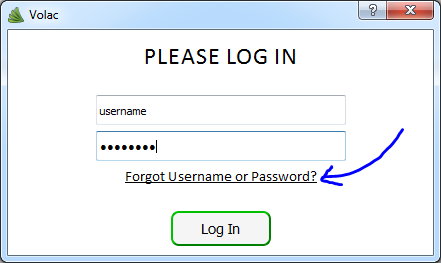
\includegraphics[width=\textwidth]{./Evaluation/Images/login4.png}
    \caption{A view of the admin "search staff" screen after member is searched.} 
\end{figure}

\begin{figure}[H]
    \includegraphics[width=\textwidth]{./Evaluation/Images/login5.png}
    \caption{A view of the admin "search staff" screen after member is searched.} 
\end{figure}



\subsection{Automatic Email}

\textbf{Objective:}The system will also have an automatic email sent to IT staff members reminding them that a warranty is running out on a particular device, this email will be sent about 3 months before the end of the warranty period.

\textbf{Has the objective been fulfilled?}

The objective has been fulfilled. When the system has been started it will check to see if any hardware warranties  are set to expire in 90 days (rounded from 3 months). If a device is going to expire an email will be sent to the email set in the system (which will be the IT Staff email). The automatic email does not work as efficiently has it could because it will not automatically work out dates while the program is running, instead it can only work out the days left if the program is restarted once a day. However most likely the program would be reset each day in a real company, but it is still a big problem that would need to be fixed at a later date. After explaining these errors to my client he stated that this needs improving on the questionnaire (question 9 \ref{qs}, page \pageref{qs}).

\textbf{Evidence}

\begin{figure}[H]
    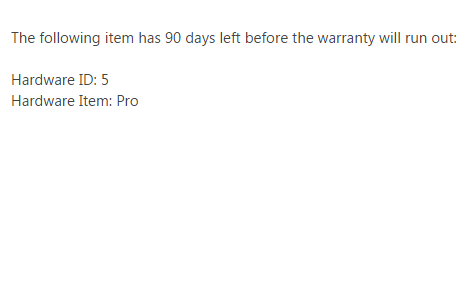
\includegraphics[width=\textwidth]{./Testing/Images/EmailExpiredHardware.png}
    \caption{This is the email received when a hardware item is about to run out of warranty.} 
\end{figure}



\subsection{Search Function}

\textbf{Objective:}The system must have a search function to allow a user to find a specific field.

\textbf{Has the objective been fulfilled?}

Objective has been fulfilled. There are search functions on every interface which enables staff to easily search the table, the user will enter text into the search box and only those fields matching the text will be shown in the table.

\textbf{Evidence}

Evidence at \ref{search} (page: \pageref{search})


\subsection{Querying Data}

\textbf{Objective:}The system must have a way to query information so that a user can filter or categorize information (such as by department or location)

\textbf{Has the objective been fulfilled?}

The objective has not been met entirely. The user can search for information (referenced in \ref{search} on page \pageref{search}) and can query staff by department. However other queries such as by location were left out, this was an optional modification to the program as there was no real need for any further queries since staff may just use the search function.

\textbf{Evidence}

Search function at \ref{search}  (page: \pageref{search})


\paragraph{Other Objectives}

\subsection{Electronic Hardware Request Forms}

\textbf{Objective:}It will be nice to include a method of sending hardware request forms electronically to eliminate the need for physical copies. However this will only be considered if everything else is completed as it is not essential.

\textbf{Has the objective been fulfilled?}

Objective has not been met. This would be a nice addition but only when the system has been fully developed.



\subsection{Online Database}

\textbf{Objective:}A great feature to have is the database being available online using the server the company owns. If the database was online it will be available to use from anywhere with internet connection.

\textbf{Has the objective been fulfilled?}

Objective has not been met. The system will not be automatically updated if it was stored on a server, also if multiple people tried to use the same system the database would be "locked" whilst in use by somebody else. 


\paragraph{Additional Objectives}

The additional objectives are not in the original specification but my client has requested them during implementation.

\textbf{Objective:}A graph to show all hardware devices in the company, split into the different departments.

\textbf{Has the objective been fulfilled?}

Objective has been met. The graph will successfully show the amount of hardware items and show how many devices each department owns. The graph can be saved by clicking the save button shown in the screenshot below. Question 15 of the questionnaire (\ref{qs}, page \pageref{qs}) strongly shows that my client thought it was successful and making a graphical representation that is easy to understand.

\textbf{Evidence}

\begin{figure}[H]
    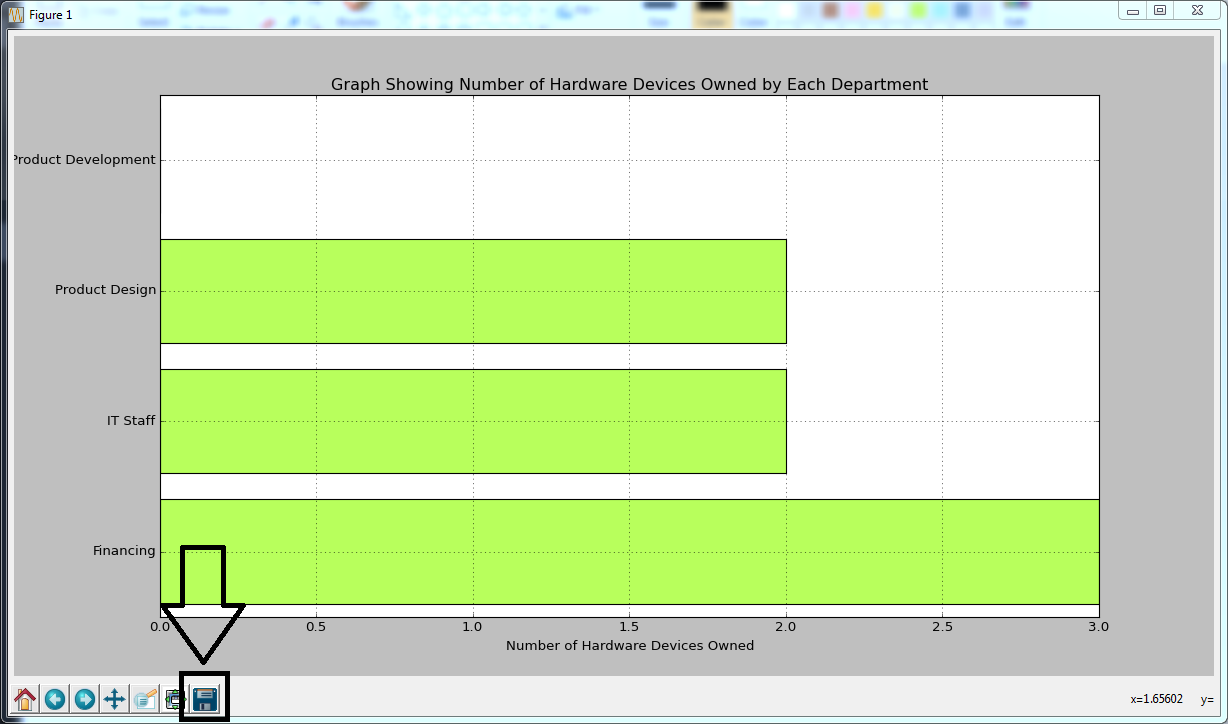
\includegraphics[width=\textwidth]{./Manual/Images/graph2.png}
    \caption{The graph display with the save button highlighted at the bottom.} 
\end{figure}

\textbf{Objective:}A clear, professional design and colour scheme that will be appealing to use for the consumers.

\textbf{Has the objective been fulfilled?}

Objective has been met. I have successfully created a colour scheme and design that my client appreciates as shown  All text is easy to read and understand and the company colours are used.

\textbf{Evidence}

\begin{figure}[H]
    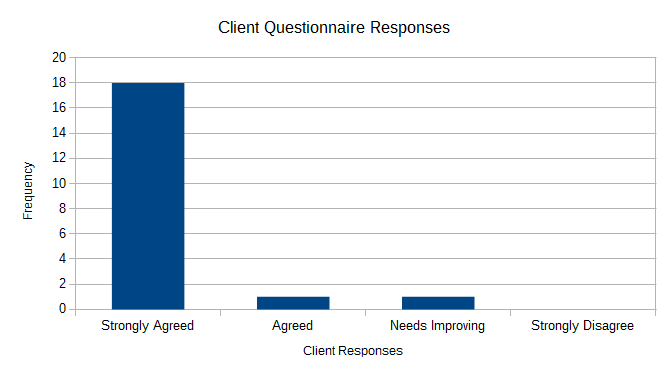
\includegraphics[width=\textwidth]{./Manual/Images/graph.png}
    \caption{An example of the main menu screen on the admin interface.} 
\end{figure}

\textbf{Objective:}Ability to send bug and incorrect information reports to keep with the Data Protection Act

\textbf{Has the objective been fulfilled?}

Objective has been met. Managers and Staff can send bug reports as well as incorrect information reports through email using the system. The emails will get sent to the IT Staff who will review the problem. 

\textbf{Evidence}

\begin{figure}[H]
    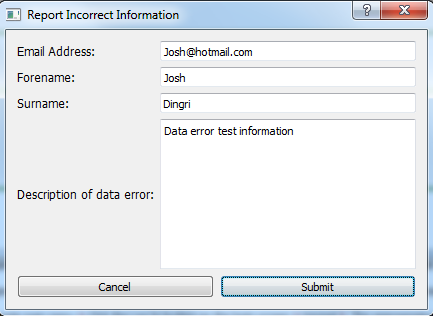
\includegraphics[width=\textwidth]{./Testing/Images/SubmitErrorReport.png}
    \caption{An example of a incorrect information report.} 
\end{figure}

\begin{figure}[H]
    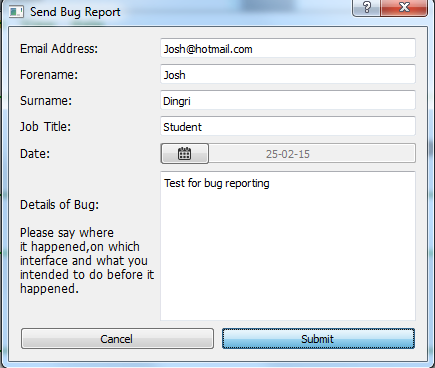
\includegraphics[width=\textwidth]{./Testing/Images/SubmitBugTest.png}
    \caption{An example of a bug report.} 
\end{figure}

\begin{figure}[H]
    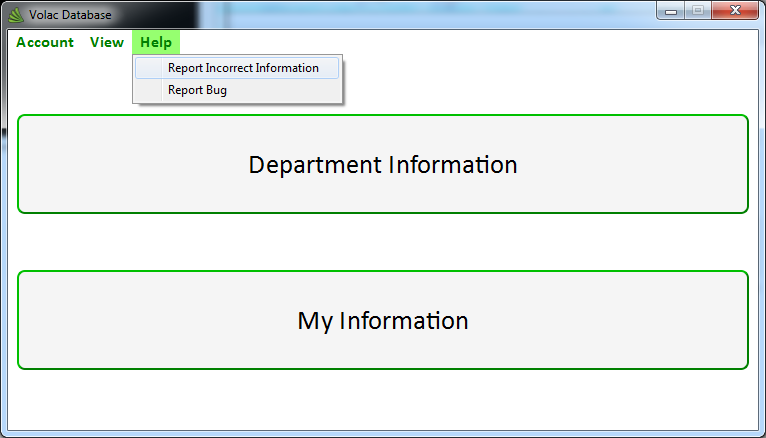
\includegraphics[width=\textwidth]{./Testing/Images/HelpMenu.png}
    \caption{Both these functions can be accessed through the help menu on the manager and staff interface.} 
\end{figure}

\textbf{Objective:}Ability to recover login details through the use of email from inside the system.

\textbf{Has the objective been fulfilled?}

The objective has been fulfilled. The system provides a way to recover login details by filling out the password recovery screen which will then send the details to the IT Staff. The IT Staff can then look at the colleagues login details and send an email back to them, alternatively they can create new login details for the colleague to use.

\begin{figure}[H]
    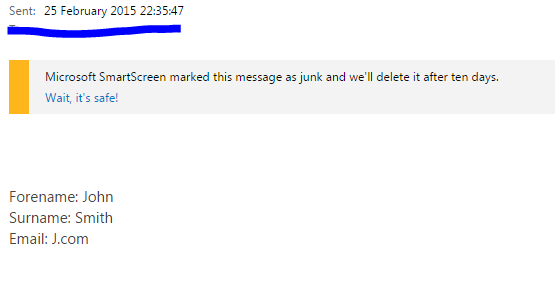
\includegraphics[width=\textwidth]{./Testing/Images/ForgotPasswordValidationEmail.png}
    \caption{An example of a password recovery email.} 
\end{figure}

\begin{figure}[H]
    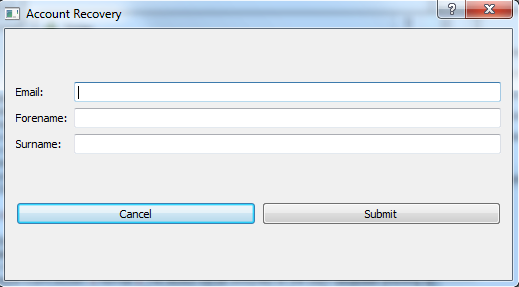
\includegraphics[width=\textwidth]{./Testing/Images/ForgotPassword.png}
    \caption{An example of a password recovery interface.} 
\end{figure}


\subsection{Summary}

Overall, the system meets most of the objectives that I set out to achieve. At some points the objective was not met, but was instead modified and improved optionally, because of this I have added a column for this in the graph shown below.

\begin{figure}[H]
    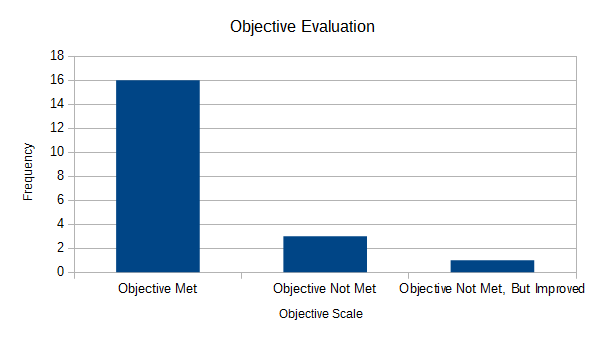
\includegraphics[width=\textwidth]{./Evaluation/EvaluationQuestionnaire/graph2.png}
    \caption{A graph to show objective evaluation} \label{graph2}
\end{figure}

As shown from the graph above 16 out of the overall 20 objectives have been met successfully. A further 1 of these objectives was modified and improved which was the search function, instead of highlighting fields the system now only shows records matching the search input. The objectives that have not been met include the sending of hardware request forms electronically and making the database online. The other objective that has not been met is the querying of data, although there is a method of querying the objective stated that there was to be multiple queries. To conclude I can say that my system meets most of the objectives that were decided in the analysis and the client is very happy with my system (shown in open question \ref{fig:q3} on page \pageref{fig:q3}).

\section{Effectiveness}

%include as many subsections as necessary for your objectives
\paragraph{General Objectives}

\subsection{Database Functionality}\label{staffhardware}

\textbf{Objective:} A database to show all current staff (with details such as their job title) and the hardware devices they are assigned to.

\textbf{Evaluation Criteria:}
\begin{itemize}
\item{Correct devices are shown}
\item{Staff can check which hardware devices they have allocated to them}
\item{Table to store staff details}
\end{itemize}

\textbf{Judgment and Evidence:}
The system has an effective way of presenting staff with their current hardware devices, the table that shows this is present of every access level since it is the core reason for the system. My client agrees that this has been effective as shown in section \ref{qs}, page \pageref{qs} question 4 and 14. The tables are organised (on the admin interface) in a drop down box and can be chosen in order to view them.

Below are the different interfaces that will present the database that shows current staff and their assigned hardware devices.

\begin{figure}[H]
    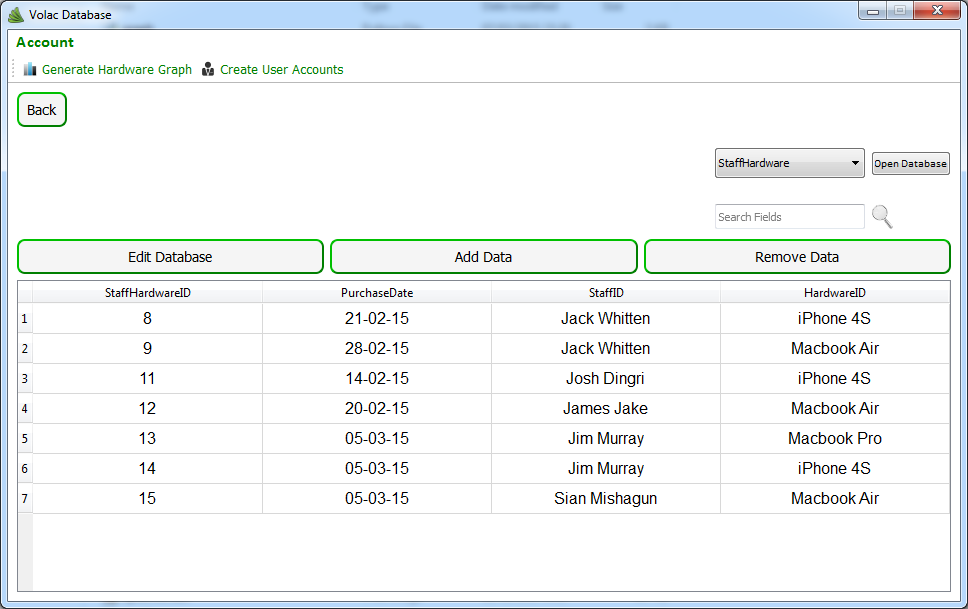
\includegraphics[width=\textwidth]{./Evaluation/Images/Database1.png}
    \caption{The Admin interface, viewing the StaffHardware Table.} \label{fig:db1}
\end{figure}

\begin{figure}[H]
    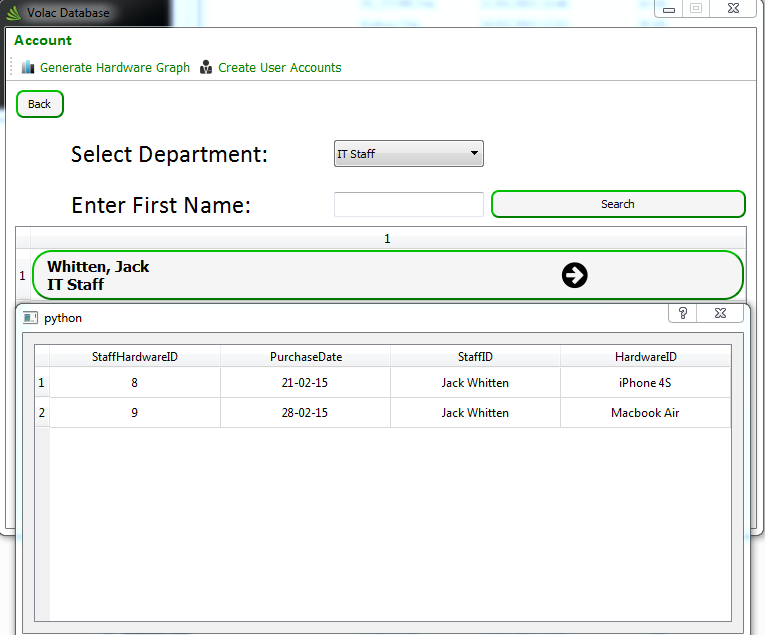
\includegraphics[width=\textwidth]{./Evaluation/Images/database3.png}
    \caption{The Admin interface: When searching for data and clicking to view more information, the StaffHardware table will appear.} \label{fig:db2}
\end{figure}

\begin{figure}[H]
    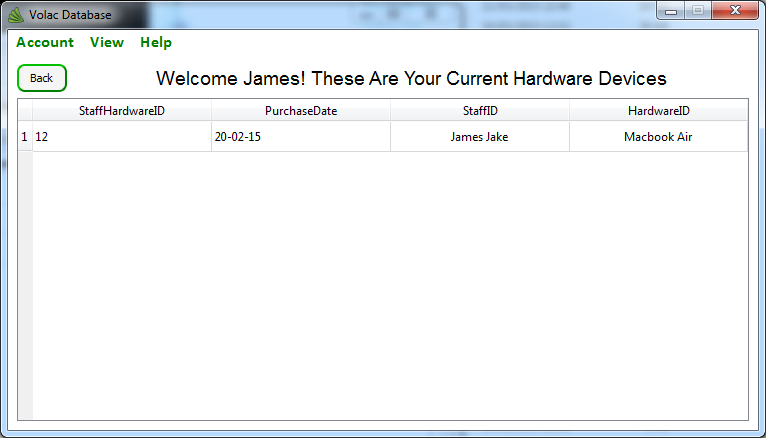
\includegraphics[width=\textwidth]{./Evaluation/Images/database2.png}
    \caption{The Manager (and staff) interface, viewing their current hardware devices.} \label{fig:db3}
\end{figure}

\subsection{Clear Database Structure}

\textbf{Objective:} The database will replace the current spreadsheet and be easy to read as information will be clear and organized.

\textbf{Evaluation Criteria:}
\begin{itemize}
\item{Tables organized and easy to read}
\item{Only necessary information shown}
\end{itemize}

\textbf{Judgment and Evidence:}

The system has all the correct fields that the original spreadsheet had (as agreed by my client \ref{qs}, page \pageref{qs} question 4) and includes more features than the current spreadsheet, therefore it will most likely replace it. Referring to question 16 of the questionnaire (\ref{qs}, page \pageref{qs}) the client has strongly agreed that the drop down box makes it easy to choose tables which shows the organisation of the system. The system is not cluttered and the buttons that are most important are large and labeled well.

\begin{figure}[H]
    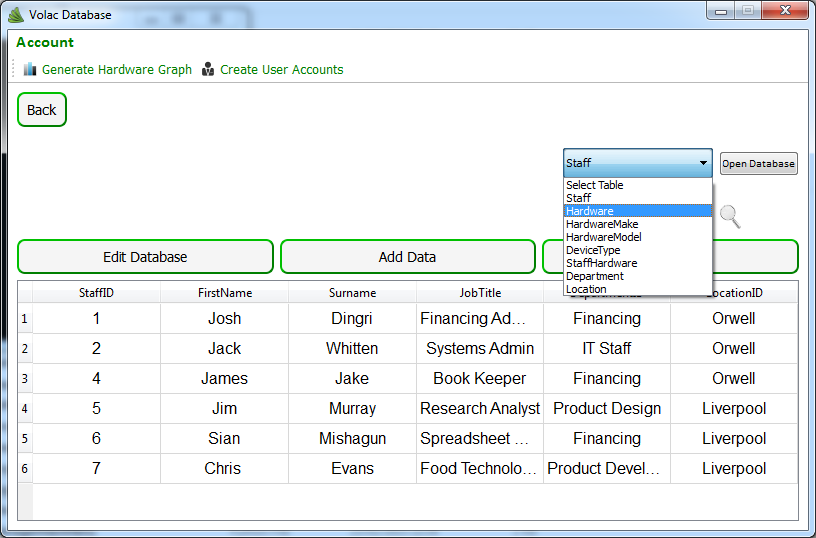
\includegraphics[width=\textwidth]{./Evaluation/Images/cleardb2.png}
    \caption{Evidence of the dropdown box to choose tables} 
\end{figure}

\subsection{Easy to use Data Input and Keyboard Shortcuts}

\textbf{Objective:} An easy to use database for IT staff to enter colleague data with toolbar buttons and keyboard shortcuts as they are advanced computer users and will want an quicker way of doing things.

\textbf{Evaluation Criteria:}
\begin{itemize}
\item{Simple keyboard shortcuts to complete tasks quicker}
\item{Use of toolbar buttons}
\end{itemize}

\textbf{Judgment and Evidence:}

The system has a number of keyboard shortcuts on the different interface, for example "CTRL+C" for changing password and "CTRL+W" to close program. According to question 5 of the questionnaire (\ref{qs}, page \pageref{qs}) my client has strongly agreed that the keyboard shortcuts allow users to complete tasks quicker. On the admin interface there are toolbar buttons to create user accounts and generate hardware graphs. However there are no toolbar buttons on the other interfaces which may have been good to include.

\begin{figure}[H]
    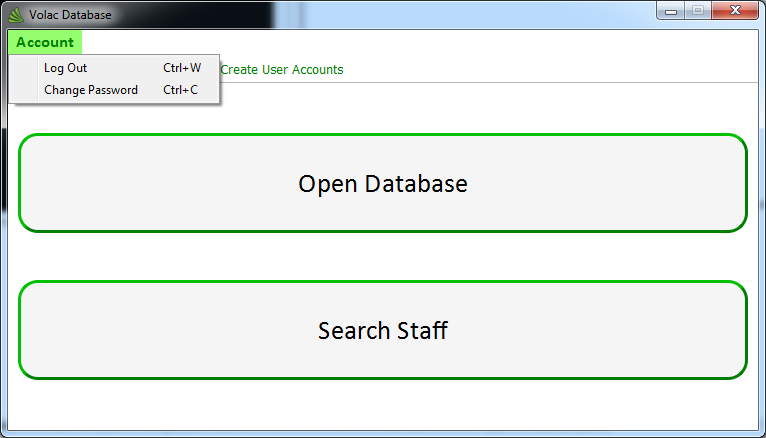
\includegraphics[width=\textwidth]{./Evaluation/Images/shortcuts1.png}
    \caption{The menu buttons can be activated by using the menubar or some (such as the above) have keyboard shortcuts attached to them.} 
\end{figure}

\begin{figure}[H]
    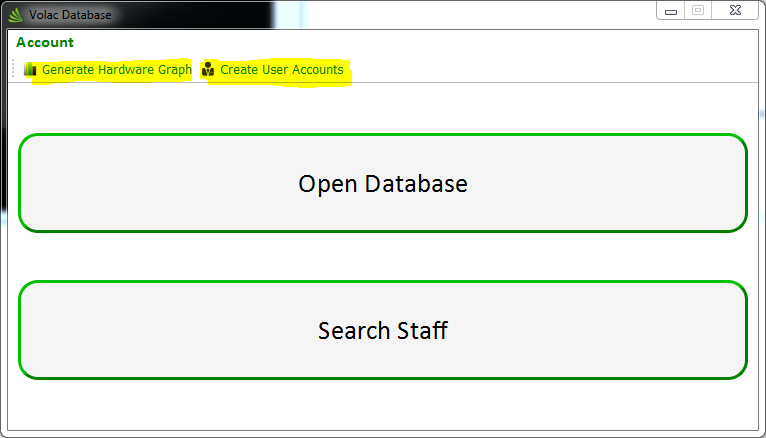
\includegraphics[width=\textwidth]{./Evaluation/Images/toolbarbtns.png}
    \caption{Example of the toolbar buttons shown on the admin interface.} 
\end{figure}

\subsection{Simple Interface Structure}

\textbf{Objective:} The layout for colleagues to see their hardware allocations will be clear and to the point, missing out any unnecessary buttons and menus.

\textbf{Evaluation Criteria:}
\begin{itemize}
\item{Simple table format for hardware allocations}
\item{Only necessary information shown}
\item{StaffHardware table (the table showing allocations) present on all interfaces}
\end{itemize}

\textbf{Judgment and Evidence:}

The table for hardware allocations to staff (staffhardware table) only has the fields: StaffHardwareID, PurchaseDate, StaffID, HardwareID. This shows that the table only shows relevant and important information and from this table staff can easily see their hardware devices. I did not include a menu from the design because it was unnecessary. For the staff interface they have a simply table showing their devices  since they do not need any extra features (as explained in \ref{interface} on page \pageref{interface}).

\begin{figure}[H]
    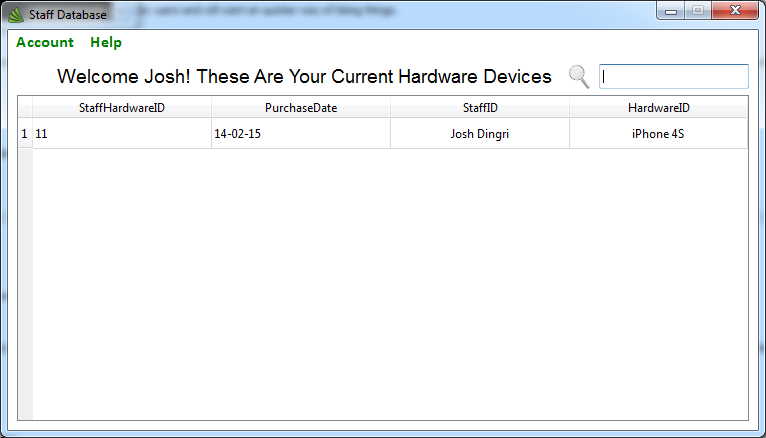
\includegraphics[width=\textwidth]{./Evaluation/Images/staffhardwaredevice.png}
    \caption{A simple view of the Staff interface showing a user's hardware items.} 
\end{figure}

\begin{figure}[H]
    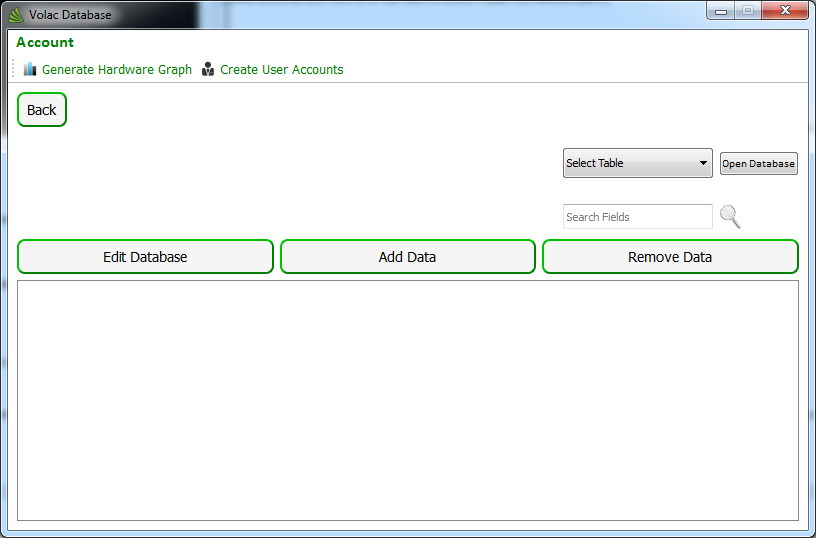
\includegraphics[width=\textwidth]{./Evaluation/Images/clearlabels.png}
    \caption{A view of the Admin interface before a database is selected. All buttons are clearly labelled and the screen is not cluttered.} 
\end{figure}

\subsection{Search Functionality}\label{searchf}

\textbf{Objective:} A search function will be in place to make searching for a field (such as staff member or hardware device) easy.

\textbf{Evaluation Criteria:}
\begin{itemize}
\item{Automatically updating search function}
\item{Easy to use and clearly labeled search box}
\end{itemize}

\textbf{Judgment and Evidence:}

The system provides an effective simple search function on all tables. It allows anything to be typed into the box and the table will instantly update showing only fields matching the search criteria. The search box also has a place holder saying "search" for the user's convenience. My client found the search function to be very effective shown in the questionnaire (\ref{qs}, page \pageref{qs}), question 17 where he strongly agreed that the search function was clear and easy to use. The advanced search (part of the admin interface, referenced at \ref{advsearch}, page \pageref{advsearch}) is done effectively but it could have improvements, during the interview for the questionnaire my client asked if it would be possible to "show all staff before selecting a specific department" (although he did not write this down on the improvements which may mean it is not essential).

Below are some examples of using the search function:

\textbf{Admin Database Screen}

\begin{figure}[H]
    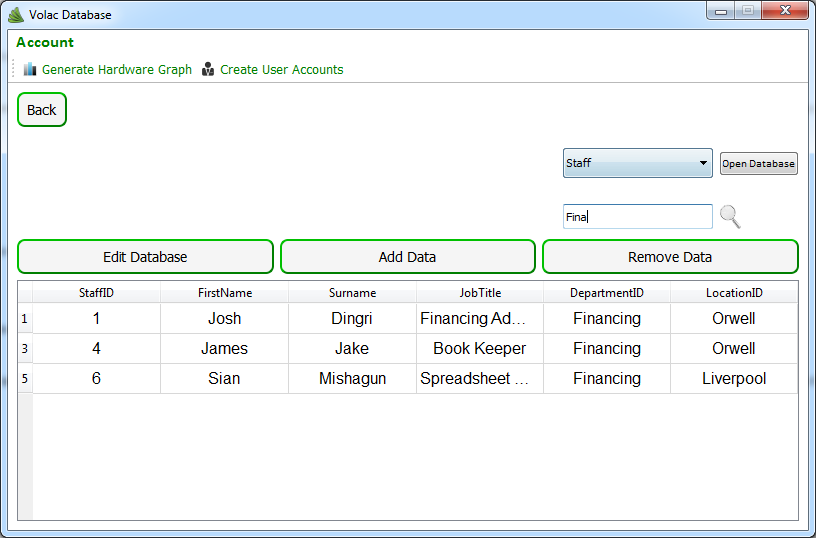
\includegraphics[width=\textwidth]{./Evaluation/Images/afteradminsearch.png}
    \caption{A view of the admin database screen after data is searched.} 
\end{figure}

\textbf{Admin Staff Search Screen}

\begin{figure}[H]
    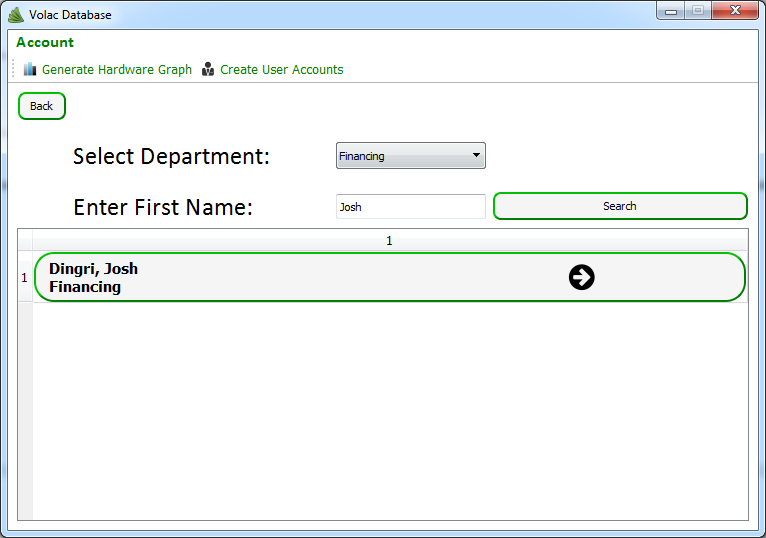
\includegraphics[width=\textwidth]{./Evaluation/Images/afteradv.png}
    \caption{A view of the admin "search staff" screen after member is searched.} \label{advsearch}
\end{figure}

\textbf{Manager Search}

\begin{figure}[H]
    \includegraphics[width=\textwidth]{./Evaluation/Images/managersearch.png}
    \caption{A view of the manager table when data is searched.} 
\end{figure}

\textbf{Staff Search}

\begin{figure}[H]
    \includegraphics[width=\textwidth]{./Evaluation/Images/staffsearch.png}
    \caption{A view of the staff table when data is searched.} 
\end{figure}

\paragraph{Specific Objectives}

\subsection{Tables}

\textbf{Objective:}The database will have one table with staff and a relationship to the table with their hardware device. This will show which hardware devices the staff are allocated and all the details of that hardware device. Staff details including department and location will be linked to the Department and Location tables.

\textbf{Evaluation Criteria:}
\begin{itemize}
\item{Effective relational database}
\item{Table showing hardware allocations}
\end{itemize}

\textbf{Judgment and Evidence:}

The StaffHardware table is what all staff will be using to check their hardware devices and is shown on every interface. The database has links between each table making it a "relational database", the "staff table" links with the "location table" and the "department table". However since it is a relational database it has foreign key IDs that can be confusing for users. In most cases I have made these IDs into actual text to make it more user friendly but when editing or deleting data these foreign IDs still appear. The client has noticed this and says in question 3  (open question) of the questionnaire \ref{qs}, page \pageref{qs} that "Record IDs would be better shown as the text associated with them".

\begin{figure}[H]
    \includegraphics[width=\textwidth]{./Testing/Images/RemoveDataButtons.png}
    \caption{Example of foreign keys being shown, which is not the most effective way to present tables.} 
\end{figure}

\subsection{How the System will Search for Data}

\textbf{Objective:}The search function will allow a user to enter text and will highlight where on the page that text is.

\textbf{Evaluation Criteria:}
\begin{itemize}
\item{Matching fields will be highlighted}
\item{Automatically updating table}
\end{itemize}

\textbf{Judgment and Evidence:}

The system improves on the objective, instead of highlighting the fields in the table, it instead will hide all records with fields not matching the search input. When I implemented the highlighted search I noticed it is very inefficient since if there were a lot of items in the table it would still take the user a while to find all the highlighted fields. Simply showing only those records that match is much easier for the user. The table will instantly updated as soon as something is typed into the search box which eliminates the need for a button. According to question 17 of the questionnaire my client strong agreed that the search function was effective and easy to use. (For more information please read \ref{searchf} on page \pageref{searchf})

\textbf{Admin Database Screen}

\begin{figure}[H]
    \includegraphics[width=\textwidth]{./Evaluation/Images/beforeadminsearch.png}
    \caption{A view of the admin database screen before any data is searched.} 
\end{figure}


\begin{figure}[H]
    \includegraphics[width=\textwidth]{./Evaluation/Images/afteradminsearch.png}
    \caption{A view of the admin database screen after data is searched.} 
\end{figure}

\subsection{Read-Only access for staff}

\textbf{Objective:} Read-Only access for staff viewing their own information (with a log-in system to allow this).

\textbf{Evaluation Criteria:}
\begin{itemize}
\item{Staff must login to access their interface}
\item{Table must be read only}
\end{itemize}

\textbf{Judgment and Evidence:}

Staff only have the StaffHardware table to view (showing allocations) and it has been set to read-only which means they can not modify the data. Admin's will create the login details for each staff member and set their access levels. My client approved of the access levels in the system as shown by question 11 in the questionnaire (\ref{qs}, page \pageref{qs}).

\begin{figure}[H]
    \includegraphics[width=\textwidth]{./Evaluation/Images/readonlymanager.png}
    \caption{The grey box around the field shows up meaning that the field cannot be modified.} 
\end{figure}

\subsection{Read-Only access for managers}

\textbf{Objective:}Read-Only access for line managers wanting to see all data about staff in their department.

\textbf{Evaluation Criteria:}
\begin{itemize}
\item{Staff must login to access their interface}
\item{Tables (including department table) must be read only}
\end{itemize}

\textbf{Judgment and Evidence:}

Managers can see their own hardware in the "My Information" screen of their interface, they can also view all hardware allocated to members of staff in their own department. Neither of these tables can be modified in any way. Again, admin's will create the login details for each manager and set their access levels.
\begin{figure}[H]
    \includegraphics[width=\textwidth]{./Evaluation/Images/readonlymanager.png}
    \caption{The grey box around the field shows up meaning that the field cannot be modified.} 
\end{figure}

\subsection{Admin access for IT Staff}\label{admin}

\textbf{Objective:}Admin rights for IT staff so they are able to view and edit all data on the database.

\textbf{Evaluation Criteria:}
\begin{itemize}
\item{Must be able to add, edit and remove data}
\item{Must be able to view all tables}
\end{itemize}

\textbf{Judgment and Evidence:}

Admin's can view all tables by selecting them from the dropdown box on the "Open Database" screen. User's can add data to any table as well as being able to remove and edit data. If an admin was to edit data in the database this is updated in the sql table so other staff can see the updated version in their interfaces. During implementation I also added the method to create user accounts which other users can log in with. Referring to question 18 of the questionnaire (\ref{qs}, page \pageref{qs}) the client has strongly agreed that data can be edited easily. Also question 19 shows that deleting data is also very easy to do for the client. When adding data I have made sure that validation and dropdown boxes make this as simple as possible, question 13 shows that I have done this successfully as my client has strongly agreed that these methods reduce human errors.

\begin{figure}[H]
    \includegraphics[width=\textwidth]{./Evaluation/Images/admin1.png}
    \caption{Admin Interface showing that all tables can be viewed in the database.} 
\end{figure}

\begin{figure}[H]
    \includegraphics[width=\textwidth]{./Evaluation/Images/admin2.png}
    \caption{Admin Interface showing that data can be edited.} 
\end{figure}

\begin{figure}[H]
    \includegraphics[width=\textwidth]{./Evaluation/Images/admin3.png}
    \caption{Admin Interface showing that data can be deleted.} 
\end{figure}

\begin{figure}[H]
    \includegraphics[width=\textwidth]{./Testing/Images/AddDataDataExample.png}
    \caption{Admin Interface showing the adding of data.} 
\end{figure}

\subsection{Querying Data}\label{queryf}

\textbf{Objective:} Users will be able to query information, for example if they wanted to show only mobile phones or if they wanted to show only specific departments.

\textbf{Evaluation Criteria:}
\begin{itemize}
\item{Must have different ways to query data}
\item{Must be able to query by department}
\end{itemize}

\textbf{Judgment and Evidence:}

The system does not have a lot of ways to query data, however the client did not seem to mention anything about this, but did mentioned that the search function is very effective (question 17 \ref{qs}, page \pageref{qs}). The only query I implemented was the search by department, this was an optional choice since any more would not have been necessary for the client since the search function is adequate. For a future update it would probably be convenient to add more ways of querying data.

The below screenshots show querying by department.

\begin{figure}[H]
    \includegraphics[width=\textwidth]{./Evaluation/Images/beforeadv.png}
    \caption{A view of the admin "search staff" screen before member is searched.} 
\end{figure}

\begin{figure}[H]
    \includegraphics[width=\textwidth]{./Evaluation/Images/afteradv.png}
    \caption{A view of the admin "search staff" screen after member is searched.} 
\end{figure}

\paragraph{Core Objectives}

\subsection{The Login System}

\textbf{Objective:}The system will provide a login system where IT staff can assign usernames to all staff and have admin rights to view all data. The database will have read-only access for colleagues viewing their own information. Managers will be able to view their departments hardware devices.

\textbf{Evaluation Criteria:}
\begin{itemize}
\item{Must have a way of admins to add user accounts}
\item{Must have three different access levels}
\item{Must have read-only access for managers and staff}
\item{managers and staff must be able to view their own hardware devices}
\end{itemize}

\textbf{Judgment and Evidence:}

Admins may add user accounts at any time by clicking the "Create User Accounts" toolbar button on any screen on the admin interface. From here they may allocate a username and password as well as setting the access restrictions for the specific member of staff. Usernames and passwords are automatically generated but can be manually changed by the admin. I have successfully created three different access levels for Staff, Managers and Admins. Each have their own interfaces with different access levels, the Staff and Managers have read-only access to the system to view their own data (mangers can also view department data). Admins have full access to the system so they can add, edit and remove data from any table.

According to question 10 of the questionnaire (\ref{qs}, page \pageref{qs}) my client was happy with the username/password format and agreed the randomly generated passwords were secure. As said in other sections above, question 10 of the questionnaire shows that my client was happy with the different access levels given to staff.


\begin{figure}[H]
    \includegraphics[width=\textwidth]{./Evaluation/Images/login1.png}
    \caption{Admin Interface showing account creation, from here they can choose access levels for other staff members to use.} 
\end{figure}

\begin{figure}[H]
    \includegraphics[width=\textwidth]{./Evaluation/Images/login2.png}
    \caption{Example of admin login.} 
\end{figure}

\begin{figure}[H]
    \includegraphics[width=\textwidth]{./Evaluation/Images/login3.png}
\end{figure}

\begin{figure}[H]
    \includegraphics[width=\textwidth]{./Evaluation/Images/login4.png}
\end{figure}

\begin{figure}[H]
    \includegraphics[width=\textwidth]{./Evaluation/Images/login5.png}
\end{figure}


\subsection{Automatic Email}

\textbf{Objective:}The system will also have an automatic email sent to IT staff members reminding them that a warranty is running out on a particular device, this email will be sent about 3 months before the end of the warranty period.

\textbf{Evaluation Criteria:}
\begin{itemize}
\item{Must send an email when hardware device is running out of warranty}
\item{Must only send the email when there is 90 days left}
\item{Should send when the program is left running}
\item{Should only send once}
\end{itemize}

\textbf{Judgment and Evidence:}

The automatic email sends successfully when there is 90 days left before the device runs out of warranty. However there are quite a few known problems that will need to be fixed. For example the email will not send if the program is left running, in order to calculate the amount of days left the program must be restarted. Obviously if this system was to be put on a server it would need to continually run, therefore the system would need to update the current date in real-time. If the program is restarted multiple times on the day that the email is being sent out it will send the email multiple times, again this is a problem.

Question 9 of the questionnaire (\ref{qs}, page \pageref{qs}) shows how my client wants the automatic email improving. Originally my client ticked the "strongly agreed" box until I explained the issues with it, it was then replaced with the "needs improving" box.

\begin{figure}[H]
    \includegraphics[width=\textwidth]{./Testing/Images/EmailExpiredHardware.png}
    \caption{This is the email received when a hardware item is about to run out of warranty.} 
\end{figure}

\subsection{Search Function}

\textbf{Objective:}The system must have a search function to allow a user to find a specific field.

See \ref{searchf} on page \pageref{searchf}  for criteria and judgement for the search function.

\subsection{Querying Data}

\textbf{Objective:}The system must have a way to query information so that a user can filter or categorize information (such as by department or location)

See \ref{queryf} on page \pageref{queryf} for criteria and judgement for querying data.



\paragraph{Other Objectives}

\subsection{Electronic Hardware Request Forms}

\textbf{Objective:}It will be nice to include a method of sending hardware request forms electronically to eliminate the need for physical copies. However this will only be considered if everything else is completed as it is not essential.

\textbf{Evaluation Criteria:}
\begin{itemize}
\item{Allow sending of hardware request forms electronically}
\item{Allow admins to receive and be able to sign off forms electronically}
\end{itemize}

\textbf{Judgment and Evidence:}

I did not manage to add this feature due to time constraints. It was important to focus on the core components of the system to ensure they were developed before the deadline. Therefore additional features, such as this, were left out of the final implementation. My client did not originally ask for this feature therefore it would have been added for convenience, he did not mention anything about this feature in the interview.

\subsection{Online Database}

\textbf{Objective:}A great feature to have is the database being available online using the server the company owns. If the database was online it will be available to use from anywhere with Internet connection.

\textbf{Evaluation Criteria:}
\begin{itemize}
\item{System should continually run on company server}
\item{Automatic emails should send without the system being restarted}
\item{Database should update whenever someone modifies data on it}
\end{itemize}

\textbf{Judgment and Evidence:}

Unfortunately the system has not been implemented to be used on a server.  During lesson there was no introduction for creating online sql tables therefore I would have needed to learn this from scratch. GUI design on desktop applications is what I have been using at home and in class, therefore this was the most sensible approach. To add this online feature I would need to research further and may implement this at a later date. My client has commented on this in the questionnaire \ref{qs}, page \pageref{qs} (question 3 of the open questions) and said he would have preferred the database to be online.

\paragraph{Additional Objectives}

The additional objectives are not in the original specification but my client has requested them during implementation.

\textbf{Objective:}A graph to show all hardware devices in the company, split into the different departments.

\textbf{Evaluation Criteria:}
\begin{itemize}
\item{Graph should be easy to read}
\item{Should show all departments and update when the database is updated}
\item{Should have a function to save the graph as an image}
\end{itemize}

\textbf{Judgment and Evidence:}

My system has met this objective very well, the graph is a adequate size so that all staff can read it easily, I have used a green colour to match the company colour scheme and also make it stand out. If an admin was to add another department to the database (which they would) the graph will automatically add that department. If the user wanted to save the image (maybe to use in a meeting) it can be done simply by clicking the save button on the graph display. My client (according to question 15 of the questionnaire \ref{qs}, page \pageref{qs}) strongly agreed that the graph is effective on showing hardware devices by department.

\begin{figure}[H]
    \includegraphics[width=\textwidth]{./Manual/Images/graph2.png}
    \caption{The graph display with the save button highlighted at the bottom.} 
\end{figure}

\textbf{Objective:}A clear, professional design and colour scheme that will be appealing to use for the consumers.

\textbf{Evaluation Criteria:}
\begin{itemize}
\item{Company colours should be used}
\item{Text should be easy to read}
\item{Design should be appealing to use}
\end{itemize}

\textbf{Judgment and Evidence:}

My system has met this objective very well, I have put a lot of effort into the overall design of my system. When choosing the colour scheme I visited the company website and matched the colours, this creates a much more professional feel to my system as the software and website match. I used a wide range of icons and images (shown on the screenshots below) as well as creating a splashscreen in photoshop that uses the company logo and a background image relating to the company image. My client really likes my design as stated on page 3 of the open questions (\ref{fig:q3} on page \pageref{fig:q3}).

\begin{figure}[H]
    \includegraphics[width=\textwidth]{./Manual/Images/graph.png}
    \caption{An example of the main menu screen on the admin interface.} 
\end{figure}

\begin{figure}[H]
    \includegraphics[width=\textwidth]{./Evaluation/Images/splashscreen.png}
 \caption{Screenshot of the splashscreen before the system loads.} 
\end{figure}

\textbf{Objective:}Ability to send bug and incorrect information reports to keep with the Data Protection Act

\textbf{Evaluation Criteria:}
\begin{itemize}
\item{Be able to send bug reports via email}
\item{Be able to send incorrect information reports via email}
\end{itemize}

\textbf{Judgment and Evidence:}

The system does this effectively, but in order to test it thoroughly I would need to use the company email server which I could not do during implementation, all staff are on the email of Volac.com but I have tested using Live.com. It should work the same, but in order to change the server I would need to modify the code slightly. The emails will be sent to a specific IT Staff email address where they can be read and investigated, the system does the correctly. My client strongly agrees that these email functions were performed effectively (questions 6 and 7 of the questionnaire \ref{qs}, page \pageref{qs}).


\begin{figure}[H]
    \includegraphics[width=\textwidth]{./Testing/Images/SubmitErrorReport.png}
    \caption{An example of a incorrect information report.} 
\end{figure}

\begin{figure}[H]
    \includegraphics[width=\textwidth]{./Testing/Images/SubmitBugTest.png}
    \caption{An example of a bug report.} 
\end{figure}

\begin{figure}[H]
    \includegraphics[width=\textwidth]{./Testing/Images/HelpMenu.png}
    \caption{Both these functions can be accessed through the help menu on the manager and staff interface.} 
\end{figure}

\textbf{Objective:}Ability to recover login details through the use of email from inside the system.

\textbf{Evaluation Criteria:}
\begin{itemize}
\item{Be able to use the system to request new login details}
\item{Using the password recovery interface an email should send to the IT Staff}
\end{itemize}

\textbf{Judgment and Evidence:}

The system provides a way to recover login details by filling out the password recovery screen which will then send the details to the IT Staff. The IT Staff can then look at the colleagues login details and send an email back to them, alternatively they can create new login details for the colleague to use. There is a problem with this solution, currently admins/IT staff cannot change another users password and the only way to see the login details would be to use sql database inspector which is very inefficient. There needs to be an improvement on the next version to allow admins to change colleagues passwords. My client ticked the strong agree box to say he thought the login detail recovery was effective (question 8 \ref{qs}, page \pageref{qs}) however he recognizes that the only way currently is to create new details for the colleague.

\begin{figure}[H]
    \includegraphics[width=\textwidth]{./Testing/Images/ForgotPasswordValidationEmail.png}
    \caption{An example of a password recovery email.} 
\end{figure}

\begin{figure}[H]
    \includegraphics[width=\textwidth]{./Testing/Images/ForgotPassword.png}
    \caption{An example of a password recovery interface.} 
\end{figure}


\section{Learnability}

Since my client is my father I had a good idea of his knowledge of working with IT systems and database. I also have good understanding of his colleagues knowledge since I have been to this company for work experience prior to developing this system. Since my client works as a Systems Administrator in the IT department of Volac his knowledge of using computers is very high therefore I did not need to add additional instructions to the system such as tooltips. The whole company works with computer systems, working on spreadsheets and databases on a daily basis. Again, this meant when developing the Manager and Staff interfaces there did not need to be basic instructions, I added shortcuts to every interface because I feel that all staff members would like quicker ways to complete tasks.

\begin{figure}[H]
    \includegraphics[width=\textwidth]{./Evaluation/Images/shortcuts2.png}
    \caption{This menu is part of the Manager interface showing F1 and F2 shortcuts which are attached to the menu buttons.} 
\end{figure}


The current spreadsheet that the IT staff use to keep track of hardware devices is much more complicated than my system, it has a lot of data duplication since it is not a relational database. Since the users would be used to this current spreadsheet I ensured that all of the important fields were copied over such as "Device Type" as well as "Location" and "Department". This has been effective since question 4 of the questionnaire (\ref{qs}, page \pageref{qs}) states that my client strongly agrees that the new system has all the correct fields needed.

\begin{figure}[H]
    \includegraphics[width=\textwidth]{./Evaluation/Images/spreadsheet.png}
    \caption{This is an example of the fields on the original spreadsheet. I have made sure to include these important fields as well as improving their names to make it more organized (Description became Device)} 
\end{figure}

When producing the search functions I researched into how searches are used in professional software. Initially I had a search button that the users had to click in order to update the table, but soon realized that it is much easier and quicker to automatically update the table whenever something is typed in. Windows 7 uses the same system in the search menu as well as Google using this autosearch in their web browser. Staff will be very used to this method so using my search function should be very straightforward.

\begin{figure}[H]
    \includegraphics[width=\textwidth]{./Evaluation/Images/afteradv.png}
    \caption{A view of the admin "search staff" screen after member is searched.}
\end{figure}

I ensured I used as many error messages as possible when designing my system, this is so users can identify that they have done something wrong and correct it instead of continually trying. However my client chose to tick "Agree" on question 20 of the questionnaire (\ref{qs}, page \pageref{qs}) instead of "Strongly Agree" this may be because he wants there to be more error messages, or to make them more obvious.

After completing the staff and manager interfaces I realized it was quite hard to tell which screen the user is currently on while navigating through these interfaces, therefore I chose to add labels to the top of each interface explaining what the screen currently shows.

\begin{figure}[H]
    \includegraphics[width=\textwidth]{./Evaluation/Images/readonlystaff.png}
    \caption{Example showing that labels on the different screens.}
\end{figure}

\begin{figure}[H]
    \includegraphics[width=\textwidth]{./Evaluation/Images/managersearch.png}
    \caption{Example showing that labels on the different screens.} 
\end{figure}

Overall referring to my above points and the client feedback it seems that my system has a fairly gradual learning curve. All users should have no problem using the system and there are labels, placeholder texts and error messages to aid the user. If someone was to use the admin interface on the system for the first time, without working on any form of database before, it may be fairly hard to grasp the relational database structure. On question 2 of the questionnaire (\ref{qs}, page \pageref{qs}) my client strongly agreed that the system was easy to use for staff inexperienced with computers, although this is a subjective view so it may not be entirely accurate.

\section{Usability}

The usability refers to how easy the system is to use, since the system has been designed with a user interface this will be the focus for the section. 

The usability can be classified by several criteria:
\begin{itemize}
\item{Target acquisition time}
\item{Latency}
\item{Readability}
\item{Use of metaphors}
\item{Navigability}
\end{itemize}

\subsection{Target acquisition time}

This refers to how long it takes to navigate around the user interface, for example how long it takes to click a certain button or choose an option from a dropdown box.

With the use of "main menus" on the manager and admin interface the target acquisition time is very low as there are two large buttons that fill the screen.

\begin{figure}[H]
    \includegraphics[width=\textwidth]{./Maintenance/Images/ManagerMM.png}
    \caption{A view of the manager main menu, showing low target acquisition time} 
\end{figure}

\begin{figure}[H]
    \includegraphics[width=\textwidth]{./Maintenance/Images/adminmainmenu.png}
    \caption{A view of the admin main menu, showing low target acquisition time} 
\end{figure}

Most of the system has very low target acquisition time, I have made sure that buttons and font is large and easily readable. 

\begin{figure}[H]
    \includegraphics[width=\textwidth]{./Evaluation/Images/beforeadv.png}
    \caption{The admin advanced search also has low target acquisition time. The buttons to view more info (with arrows) are very large with bold text making them easily readable.} 
\end{figure}

There is however one part of the system that has higher target acquisition time. When editing data the font is smaller and may be hard to select fields (shown below).

\begin{figure}[H]
    \includegraphics[width=\textwidth]{./Evaluation/Images/admin2.png}
\end{figure}

\subsection{Latency}

Latency refers to how long after an action has been initiated the system takes to complete it. Latency seems to be a problem when first starting the program (particularly on slow computers), there is around a three second pause before the splashscreen is shown. However every action is performed almost instantly on the rest of the system.

\subsection{Readability}

Readability refers to how easy is it for a user to read commands or guidance. The readability of my system is generally very good, the system has been designed with the company colours of green/white with black text. The black text stands out very well on the white background. The font is large so it can be read easily and for important text, bold is used.

\begin{figure}[H]
    \includegraphics[width=\textwidth]{./Evaluation/Images/managersearch.png}
    \caption{Example of bold, large labels on the manager interface.} 
\end{figure}

However has referenced in target acquisition time, the readability of the fields when editing data is very low as the font size is much smaller.

\begin{figure}[H]
    \includegraphics[width=\textwidth]{./Evaluation/Images/admin2.png}
\end{figure}

\subsection{Use of metaphors}

The use of metaphors is if there are visual pictures or icons to help users understand what can be done. I have included a variety of icons and pictures in my system, for some this was simply added to make the system more appealing and nicer to use. However the calendar icon has a button attached to it that will be clicked in order to choose a date. Below are some examples of where pictures and icons are used in my system.

\begin{figure}[H]
    \includegraphics[width=\textwidth]{./Evaluation/Images/toolbaricons.png}
    \caption{These icons are linked with the toolbar button and provide a visual aid as well as the text format, this should help the user work out what the buttons do.} 
\end{figure}

\begin{figure}[H]
    \includegraphics[width=\textwidth]{./Evaluation/Images/arrowicon.png}
    \caption{The arrow picture was used here because it shows that clicking the button will open a new interface.} 
\end{figure}

\begin{figure}[H]
    \includegraphics[width=\textwidth]{./Evaluation/Images/calandericon.png}
    \caption{The calendar icon on this screen will need to be clicked to choose a date.} 
\end{figure}

\begin{figure}[H]
    \includegraphics[width=\textwidth]{./Evaluation/Images/calandericon2.png}
    \caption{The calendar after the icon has been clicked.} 
\end{figure}

There are also icons and pictures that help with the design of the system. For example the splash screen shown below does not change how the system functions but makes it look much more professional.

\begin{figure}[H]
    \includegraphics[width=\textwidth]{./Evaluation/Images/splashscreen.png}
\end{figure}

I have also added an icon for the system that will show on the taskbar on windows as well as the executable file and the top left corner of the application.

\begin{figure}[H]
    \includegraphics[width=\textwidth]{./Evaluation/Images/volacicon.png}
\end{figure}

\begin{figure}[H]
    \includegraphics[width=\textwidth]{./Evaluation/Images/volacicon2.png}
\end{figure}

\begin{figure}[H]
    \includegraphics[width=\textwidth]{./Evaluation/Images/volacicon3.png}
\end{figure}

Overall the use of metaphors is a very large part of my system as I believe that it should look as professional as possible, and be appealing to use for staff since they will be using it a lot.

\subsection{Navigability}

This section is looking at how easy it is to navigate the user interface. I believe that my system is fairly simple to navigate through, as mentioned earlier I have main menu screens for Managers and Admins (as they have multiple interfaces) and from here there are two large buttons which go to the two interface screens. All buttons on the system are labeled and there are often multiple ways to complete a task. For navigating to department information (manager interface) the user may use the shortcut key F1, use the menu button, or use the main menu button. There are also back buttons on every screen to navigate back to the main menu, this is a design that is common on a lot of software and my client will recognise this design. According to my client (questionnaire \ref{qs}, page \pageref{qs} question 1) it was easy to navigate to the search staff screen, and when asked if there were any interfaces that were hard to navigate to he left no comments. 

During testing (see Testing section, series 1) my user interface passed every test without any errors which strongly shows its navigability. Overall I believe that the navigability of the system is very straightforward and one of the strongest parts of the system, it shouldn't have any negative impact on the usability.

\subsection{Summary}

Overall, I would say that the usability of the system is very good. My main strengths are with the use of metaphors and the navigability. The target acquisition time and readability are a little reduced due to the small font on the edit data interface, however it does not reduce the usability by that much to make it a problem. The latency upon startup is an issue on slow machines, but since the company's computers have relatively fast processors, this hopefully wont be too much of an issue.

\section{Maintainability}

The maintainability refers to three tasks:

\begin{itemize}
\item{Fixing bugs}
\item{Changing parameters}
\item{Responding to new requirements}
\end{itemize}

\subsection{Fixing Bugs}

I have tried to make my code as easy as possible for another programmer to modify or add to. Only a small number of bugs exist in my program but it is important that they can be fixed easily. I have taken the follow steps to ensure that any bugs can be fixed easily:
\begin{itemize}
\item{I have made sure that my code is self-documented and it should be relatively easy to follow. Therefore if a bug was to arise, it should be fairly straightforward for a programmer to identify and fix the errors (see System Maintenance - Section 4.10, Page 338)}
\item{I have included comments with complicated sections of code to help a programmer understand what is going on. Doc strings are also used on some functions and classes to give a summary of what they do.  (see System Maintenance - Section 4.10.1, Page 339)}
\item{See the System Maintenance section for further documentation and code examples (Pages 267-475). Section 4.7.1 of the System Maintenance provides explanation of difficult sections of code, this will definitely help and maintainer of my code.}
\end{itemize}

\subsection{Changing Parameters}

In some circumstances certain parameters in the code will need to be changed. For example if the company was to change the database file name from "Volac.db" they would need to change all of the sql queries with that parameter. Should a change be needed, it should be fairly straightforward for the following reasons:
\begin{itemize}
\item{The code is well commented, as well as certain functions having doc strings. Therefore the maintainer will easily be able to understand variables, parameters and procedures (see System Maintenance Section 4.10, Page 338)}
\item{The System Maintenance section explains the majority of my code in great detail. The variable listing (section 4.4, page 281) explains what all the important variables do in the system. Following section 4.7.1 of the System Maintenance may also help since it explains the complex parts of my code as well as the parameters and variables.}
\end{itemize}

\subsection{Responding to New Requirements}

The system should be relatively easy to adapt to new requirements, new fields can be added very easily because of the relational structure of the database, however adding fields to existing data may be quite challenging. Adding new buttons and functions to the system should fairly straightforward as there is room to do this. Below are some points to consider when adapting the system to respond to new requirements.
\begin{itemize}
\item{I have split my system into a lot of different modules that all will perform different tasks, therefore to alter the system, the user should only need to alter one module (see section 4.10 System Maintenance, Page 338)}
\item{The code is self-documented, the variable names have been carefully chosen so the code is easily readable for another programmer (see section 4.10 System Maintenance, Page 338)}
\item{There are comments to explain complex areas of code, therefore sections are clearly explained for other programmers  (see section 4.10 System Maintenance, Page 338)}
\item{The program is split into classes and methods, each method can therefore be testing individually which makes testing these new alterations easier and faster (see section 4.10 System Maintenance, Page 338)}
\item{The System Maintenance section (Pages 267-475) provides detailed code explanations as well variable listings and sql queries. Algorithms and entity relationships are also shown in this section. A maintainer of my system should be able to learn a lot from this section and understand how hard it will be to implement a new feature}
\end{itemize}

\subsection{Summary}

Overall, the system has a good level maintainability. It does this especially through the use of self-documented code, comments and doc strings which make it easy for a programmer to understand my code. The program does include quite a lot of local variables with parameters but as an improvement it may be useful to include even more so that responding to new requirements can be done easier without affecting the rest of the system.

\section{Suggestions for Improvement}

My client did largely agreed that my system was very efficient and an effective way to organise hardware allocations of staff members at Volac. The last open question on the questionnaire (\ref{fig:q3}, page \pageref{fig:q3}) asks if the user has any further comments, to which my client replied "it is a great utility that we can use to replace our spreadsheet". However there were also some improvements that he would like to see on future versions of the system. There were not many improvements that he would like added, but the ones he stated are listed below.

\subsection{Online functionality for the database}

This is by far the most desirable improvement the client would like me to add to my system. According to question 3 (open question) on page \pageref{fig:q1} my client said an improvement would be a "cloud based online version as it would allow staff to add/review hardware from anywhere". He recognizes that it was a challenge to add for this system version but would be ideal for later improvements.

\subsection{User-friendly foreign keys}

I explained how the relational database works and pointed out that when editing and removing records these foreign keys are shown. According to question 3 (open question) on page \pageref{fig:q1} my client stated that "Record IDs would be better shown as the text associated with them". Although he obviously understands how the foreign keys work it shows that they are still not user friendly and will need to have the text variant shown instead.

\subsection{Dialog Box Improvements}

On page 2 of the open questions (\ref{fig:q2} page \pageref{fig:q2}) my client requested an improvement to the current dialog boxes when sending emails. Currently when the user clicks "send" or "submit" the dialog box stays open when the email has been sent. My client asked if the dialog box could close automatically after the email is sent, otherwise users would not know if the email has sent or not. This is a very feasible improvement and I will make sure to include it in the next software version.


\section{End User Evidence}

Below is my questionnaire. The first couple of pages are closed questions were the client is required to tick a box on how strongly they agree that the particular objective has been met. The next three pages are open questions, the number before the question is the closed question it links to. 

\subsection{Questionnaire}\label{qs}

\begin{figure}[H]
    \includegraphics[width=120mm,scale=1]{./Evaluation/EvaluationQuestionnaire/Scan9.jpeg}
    \caption{Questionnaire Closed Questions: Page 1} 
\end{figure}

\begin{figure}[H]
    \includegraphics[width=\textwidth]{./Evaluation/EvaluationQuestionnaire/Scan11.jpeg}
    \caption{Questionnaire Closed Questions: Page 2}
\end{figure}

\begin{figure}[H]
    \includegraphics[width=\textwidth]{./Evaluation/EvaluationQuestionnaire/Scan12.jpeg}
    \caption{Questionnaire Open Questions: Page 1} \label{fig:q1}
\end{figure}

\begin{figure}[H]
    \includegraphics[width=\textwidth]{./Evaluation/EvaluationQuestionnaire/Scan13.jpeg}
    \caption{Questionnaire Open Questions: Page 2} \label{fig:q2}
\end{figure}

\begin{figure}[H]
    \includegraphics[width=\textwidth]{./Evaluation/EvaluationQuestionnaire/Scan14.jpeg}
    \caption{Questionnaire Open Questions: Page 3} \label{fig:q3}
\end{figure}

\subsection{Graphs}

\begin{figure}[H]
    \includegraphics[width=\textwidth]{./Evaluation/EvaluationQuestionnaire/graph.png}
    \caption{A graph to summaries the closed question feedback from my client} \label{graph}
\end{figure}

\begin{figure}[H]
    \includegraphics[width=\textwidth]{./Evaluation/EvaluationQuestionnaire/graph2.png}
    \caption{A graph to show objective evaluations} \label{graph2}
\end{figure}

